
\documentclass[a4paper,10pt]{book}
\usepackage{graphics}
\usepackage{boxedminipage}
\usepackage[colorlinks=true,urlcolor=blue]{hyperref}
\usepackage{fancyhdr}
\usepackage{fancyvrb}
\usepackage{makeidx}
\usepackage{graphicx}
\usepackage{garamond}
\usepackage{lmodern}
\usepackage[T1]{fontenc}
\usepackage{enumerate}

\title{XtreemFS Installation and User Guide}

\setlength{\parindent}{0pt}
\setlength{\parskip}{1ex plus 0.5ex minus 0.2ex}

\makeindex

\begin{document}
\pagenumbering{roman}
\begin{titlepage}
\begin{flushright}
 
\includegraphics{images/final_logo.pdf}
 % final_logo.pdf: 192x56 pixel, 72dpi, 6.77x1.98 cm, bb=0 0 192 56
\end{flushright}

\vspace{3cm}

\begin{flushleft}
\sffamily \begin{LARGE}The XtreemFS Installation and User Guide\end{LARGE}

Version 1.3.x
\end{flushleft}


\end{titlepage}
\garamond
XtreemFS is available from the \href{http://www.XtreemFS.org}{XtreemFS website (www.XtreemFS.org)}.


This document is \copyright{} 2009-2011 by Bj\"orn Kolbeck, Jan Stender, Michael Berlin, Paul Seiferth, Felix Langner, NEC HPC Europe, Felix Hupfeld, Juan Gonzales. All rights reserved.

\setcounter{tocdepth}{10}
\tableofcontents

\chapter*{Changes}
Summary of important changes in release 1.3:

\begin{itemize}
 \item \textbf{new client}\\
 We have re-written the client from scratch. The new client supports automatic fail-over for replicated files and metadata caching.
 \item \textbf{libxtreemfs}\\
 libxtreemfs is a convenient C++ library to use XtreemFS directly without a mounted client or the VFS layer. The new client is built on top of this library. A java version of libxtreemfs is planned.
 \item \textbf{File system snapshots}\\
 XtreemFS now supports snapshots. A snapshot reflects a momentary state of a volume or directory. It can be mounted and read-only accessed.
 \item \textbf{Full file replication}\\
 Starting with this release, XtreemFS supports full file replication. Read/write replicated files offer regular file system semantics and work with all applications.
 \item \textbf{DIR, MRC replication}\\
 The DIR and MRC can now be replicated using the BabuDB database replication. The replication works with a primary and backups. If the primary fails, a backup will automatically take over after a short time.
 \item \textbf{xtfsutil}\\
 We have replaced all user tools with a single binary. The new tool doesn't require java anymore.
 \item \textbf{OSD drain}\\
 With OSD drain, files can be removed from an OSD without interrupting the system. A fully drained OSD can be removed from the system without data loss.
\end{itemize}

Summary of important changes in release 1.2.1:

\begin{itemize}
 \item \textbf{server status}\\
 Each server (especially OSDs) have a persistent status which can be online or dead/removed. This status must be changed manually and is used by the scrubber tool to identify dead OSDs which have been removed from the system.
 \item \textbf{enhanced scrubber}\\
 The scrubber is now able to remove replicas which are stored on OSDs that are marked as dead/removed. The scrubber will create new replicas for that file if a complete replica still exists and a sufficient number of OSDs is available. In addition, the scrubber marks replicas as ``complete'' if they contain all objects of the original file.
\end{itemize}


This is a summary of the most important changes in release 1.2:

\begin{itemize}
 \item \textbf{renamed binaries}\\
 We renamed most binaries to conform with Linux naming conventions, e.g. \texttt{xtfs\_mount} is now \texttt{mount.xtreemfs}. However, we added links with the old names for compatibility. For a full list see Sec. \ref{sec:cli_utils}. 

 \item \textbf{``Grid SSL'' mode}\\
 In this mode, SSL is only used for authentication (handshake) and regular TCP is used for communication afterwards. For more details see Sec. \ref{sec:cfg_ssl}.

 \item \textbf{the \texttt{xctl} utility}\\
 The new release includes a command line utility \texttt{xctl} for starting and stopping the services. This tool is useful if you don't want a package based installation or if you don't have root privileges.

 \item \textbf{vivaldi}\\
 XtreemFS now includes modules for calculating Vivaldi network coordinates to reflect the latency between OSDs and clients. An OSD and replica selection policy for vivaldi is also available. For details, see Sec. \ref{sec:vivaldi}.

\end{itemize}


\chapter{Quick Start}
\label{sec:quick_start}

This is the very short version to help you set up a local installation of XtreemFS.

\begin{enumerate}
 \item Download XtreemFS RPMs/DEBs and install
	\begin{enumerate}
		\item Download the RPMs or DEBs for your system from the XtreemFS website (\href{http://www.xtreemfs.org}{http://www.xtreemfs.org})
		\item open a root console (\texttt{su} or \texttt{sudo})
		\item install with \texttt{rpm -Uhv xtreemfs*-1.3.x.rpm}
	\end{enumerate}
\item Start the Directory Service:\\
	\texttt{/etc/init.d/xtreemfs-dir start}
\item Start the Metadata Server:\\
	\texttt{/etc/init.d/xtreemfs-mrc start}
\item Start the OSD:\\
	\texttt{/etc/init.d/xtreemfs-osd start}

\item If not already loaded, load the FUSE kernel module:\\
	\texttt{modprobe fuse}

\item Depending on your distribution, you may have to add users to a special group to allow them to mount FUSE file systems. In openSUSE users must be in the group \texttt{trusted}, in Ubuntu in the group \texttt{fuse}. You may need to log out and log in again for the new group membership to become effective.

\item You can now close the root console and work as a regular user.

\item Wait a few seconds for the services to register at the directory service. You can check the registry by opening the DIR status page in your favorite web browser \href{http://localhost:30638}{http://localhost:30638}.

\item Create a new volume with the default settings:\\
	\texttt{mkfs.xtreemfs localhost/myVolume}

\item Create a mount point:\\
	\texttt{mkdir \~{}/xtreemfs}

\item Mount XtreemFS on your computer:
	\begin{verbatim}
	mount.xtreemfs localhost/myVolume ~/xtreemfs
	\end{verbatim}


\item Have fun ;-)

\item To un-mount XtreemFS:\\
	\texttt{umount.xtreemfs \~{}/xtreemfs}
\end{enumerate}

You can also mount this volume on remote computers. First make sure that the ports 32636, 32638 and 32640 are open for incoming TCP connections. You must also specify a hostname that can be resolved by the remote machine! This hostname has to be used instead of \texttt{localhost} when mounting.

\chapter{About XtreemFS}
\pagenumbering{arabic}
\setcounter{page}{1}

Since you decided to take a look at this user guide, you probably read or heard about XtreemFS and want to find out more. This chapter contains basic information about the characteristics and the architecture of XtreemFS.

\section{What is XtreemFS?}
XtreemFS is a file system for a variety of different use cases and purposes. Since it is impossible to categorize or explain XtreemFS in a single sentence, we introduce XtreemFS by means of its two most significant properties: \emph{XtreemFS is a globally distributed and replicated file system.}

\paragraph{What makes XtreemFS a distributed file system?} We consider a file system as \emph{distributed} if files are stored across a number of servers rather than a single server or local machine. Unlike local or network file systems, a distributed file system aggregates the capacity of multiple servers. As a \emph{globally distributed} file system, XtreemFS servers may be dispersed all over the world. The capacity can be increased and decreased by adding and removing servers, but from a user's perspective, the file system appears to reside on a single machine.

\paragraph{What makes XtreemFS a replicated file system?} We call it a \emph{replicated} file system because replication is one of its most prominent features. XtreemFS is capable of maintaining replicas of files on different servers. Thus, files remain accessible even if single servers, hard disks or network connections fail. Besides, replication yields benefits in terms of data rates and access times. Different replicas of a file can be accessed simultaneously on different servers, which may lead to a better performance compared to simultaneous accesses on a single server. By placing file replicas close the consuming users and applications in a globally distributed installation, the effects of network latency and bandwidth reduction in wide area networks can be mitigated. However, replication is transparent to users and applications that work with XtreemFS; the file system is capable of controlling the life cycle and access of replicas without the need for human intervention or modifications of existing applications.

\section{Is XtreemFS suitable for me?}
If you consider using XtreemFS, you may be a system administrator in search of a better and more flexible alternative to your current data management solution. Or you may be a private user in need of a file system that can be easily set up and accessed from any machine in the world. You might also be someone looking for an open-source solution to manage large amounts of data distributed across multiple sites. In any case, you will wonder if XtreemFS fulfills your requirements. As a basis for your decision, the following two paragraphs point out the characteristics of XtreemFS.

\paragraph{XtreemFS is ...}
\begin{itemize}
 \item [...] an open source file system. It is distributed freely and can be used by anyone without limitations.
 \item [...] a POSIX file system. Users can mount and access XtreemFS like any other common file system. Application can access XtreemFS via the standard file system interface, i.e.\ without having to be rebuilt against a specialized API. XtreemFS supports a POSIX-compliant access control model.
 \item [...] a multi-platform file system. Server and client modules can be installed and run on different platforms, including most Linux distributions, Solaris, Mac OS X and Windows.
 \item [...] a globally distributed file system. Unlike cluster file systems, an XtreemFS installation is not restricted to a single administrative domain or cluster. It can span the globe and may comprise servers in different administrative domains.
 \item [...] a failure-tolerant file system. As stated in the previous section, replication can keep the system alive and the data safe. In this respect, XtreemFS differs from most other open-source file systems.
 \item [...] a secure file system. To ensure security in an untrusted, worldwide network, all network traffic can be encrypted with SSL connections, and users can be authenticated with X.509 certificates.
 \item [...] a customizable file system. Since XtreemFS can be used in different environments, we consider it necessary to give administrators the possibility of adapting XtreemFS to the specific needs of their users. Customizable policies make it possible change the behavior of XtreemFS in terms of authentication, access control, striping, replica placement, replica selection and others. Such policies can be selected from a set of predefined policies, or implemented by administrators and plugged in the system.
\end{itemize}

\paragraph{XtreemFS is not ...}
\begin{itemize}
 \item [...] a high-performance cluster file system. Even though XtreemFS reaches acceptable throughput rates on a local cluster, it cannot compete with specialized cluster file systems in terms of raw performance numbers. Most such file systems have an optimized network stack and protocols, and a substantially larger development team. If you have huge amounts of data on a local cluster with little requirements but high throughput rates to them, a cluster file system is probably the better alternative.
 \item [...] a replacement for a local file system. Even though XtreemFS can be set up and mounted on a single machine, the additional software stack degrades the performance, which makes XtreemFS a bad alternative.
 %\item [...] a commercially supported product, so far. XtreemFS is being developed as part of the XtreemOS project, a research project funded by the European commission. Even though we do not want to rule out the possibility of providing commercial support for XtreemFS in the future, we currently see ourselves as researchers rather than professional file system developers.
\end{itemize}

\section{Core Features}
The core functionality of XtreemFS is characterized by a small set of features, which are explained in the following.

\paragraph{Distribution.}
An XtreemFS installation comprises multiple servers that may run on different nodes connected on a local cluster or via the Internet. Provided that the servers are reachable, a client module installed on any machine in the world can access the installation. A binary communication protocol based on Google's Protocol Buffers ensures an efficient communication with little overhead between clients and servers. XtreemFS ensures that the file system remains in a consistent state even if multiple clients access a common set of files and directories. Similar to NFS, it offers a close-to-open consistency model in the event of concurrent file accesses.

\paragraph{Replication.}
Starting with release 1.3, XtreemFS supports the replication of mutable files as well as a replicated Directory Service (DIR) and Metadata Catalog (MRC). All components in XtreemFS can be replicated for redundancy which results in a fully fault-tolerant file system. The replication in XtreemFS works with hot backups, which automatically take over if the primary replica fails.

Since version 1.0, XtreemFS supports \emph{read-only replication}. A file may have multiple replicas, provided that the it was explicitly made read-only before, which means that its content cannot be changed anymore. This kind of replication can be used to make write-once files available to many consumers, or to protect them from losses due to hardware failures. Besides complete replicas that are immediately synchronized after having been created, XtreemFS also supports partial replicas that are only filled with content on demand. They can e.g.\ be used to make large files accessible to many clients, of which only parts need to be accessed.

\paragraph{Striping.}
To ensure acceptable I/O throughput rates when accessing large files, XtreemFS supports \emph{striping}. A striped file is split into multiple chunks (``\emph{stripes}''), which are stored on different storage servers. Since different stripes can be accessed in parallel, the whole file can be read or written with the aggregated network and storage bandwidth of multiple servers. XtreemFS currently supports the \texttt{RAID0}\index{RAID0} striping pattern, which splits a file up in a set of stripes of a fixed size, and distributes them across a set of storage servers in a round-robin fashion. The size of an individual stripe as well as the number of storage servers used can be configured on a per-file or per-directory basis.

\paragraph{Security.}
To enforce security, XtreemFS offers mechanisms for user authentication and authorization, as well as the possibility to encrypt network traffic.

\emph{Authentication} \index{Authentication} describes the process of verifying a user's or client's identity. By default, authentication in XtreemFS is based on local user names and depends on the trustworthiness of clients and networks. In case a more secure solution is needed, X.509 certificates can be used.

\emph{Authorization}\index{Authorization} describes the process of checking user permissions to execute an operation. XtreemFS supports the standard UNIX permission model, which allows for assigning individual access rights to file owners, owning groups and other users.

Authentication and authorization are policy-based, which means that different models and mechanisms can be used to authenticate and authorize users. Besides, the policies are pluggable, i.e.\ they can be freely defined and easily extended.

XtreemFS uses unauthenticated and unencrypted TCP connections by default. To encrypt all network traffic, services and clients can establish \emph{SSL}\index{SSL} connections. However, using SSL requires that all users and services have valid X.509\index{X.509}\index{Certificate} certificates.

%When using XtreemFS as part of an \emph{XtreemOS} installation, users can benefit from a transparent integration with the XtreemOS \emph{Virtual Organization (VO)} infrastructure in the form of dynamic user mappings and automatic mounting of home volumes.

\section{Architecture}
XtreemFS implements an \emph{object-based file system architecture}\index{Object-based File System}\index{Architecture} (Fig. \ref{fig:architecture}): file content is split into a series of fixed-size \emph{objects}\index{Object} and stored across storage servers, while \emph{metadata}\index{Metadata} is stored on a separate metadata server. The metadata server organizes file system metadata as a set of \emph{volumes}\index{Volume}, each of which implements a separate file system namespace in the form of a directory tree.

In contrast to block-based file systems, the management of available and used storage space is offloaded from the metadata server to the storage servers. Rather than inode lists with block addresses, file metadata contains lists of storage servers responsible for the objects, together with striping policies\index{Striping Policy}\index{Policy!Striping Policy} that define how to translate between byte offsets and object IDs. This implies that object sizes may vary from file to file.

%The advantage of this architecture is that the read and write operations, which make up 80 to 90 \% of all requests, can be spread across a large number of storage servers.

\begin{figure}
 \centering
 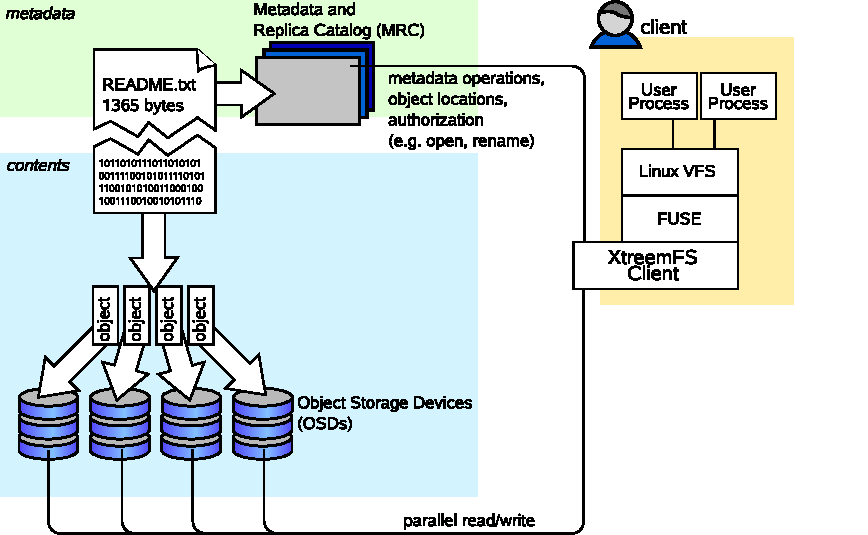
\includegraphics[width=\textwidth]{images/architecture.pdf}
 % architecture.pdf: 417x257 pixel, 72dpi, 14.71x9.07 cm, bb=0 0 417 257
 \caption{The XtreemFS architecture and components.}
 \label{fig:architecture}
\end{figure}


\paragraph{XtreemFS Components.}
An XtreemFS installation contains three types of servers that can run on one or several machines (Fig. \ref{fig:architecture}):

\begin{itemize}
 \item DIR - Directory Service\index{DIR}\index{Directory Service}\\
 The directory service is the central registry for all services in XtreemFS. The MRC uses it to discover storage servers.
 \item MRC - Metadata and Replica Catalog\index{MRC}\index{Metadata Server}\index{Metadata and Replica Catalog}\\
 The MRC stores the directory tree and file metadata such as file name, size or modification time. Moreover, the MRC authenticates users and authorizes access to files.
 \item OSD - Object Storage Device\index{OSD}\index{Storage Server}\index{Object Storage Device}\\
 An OSD stores arbitrary objects of files; clients read and write file data on OSDs.
\end{itemize}

These servers are connected by the \emph{client}\index{Client} to a file system. A client \emph{mounts}\index{Mounting} one of the volumes\index{Volume} of the MRC in a local directory. It translates file system calls into RPCs sent to the respective servers.

The client is implemented as a \emph{FUSE user-level driver} that runs as a normal process. FUSE\index{FUSE} itself is a kernel-userland hybrid that connects the user-land driver to Linux' \emph{Virtual File System (VFS)}\index{VFS} layer where file system drivers usually live.


\chapter{XtreemFS Services}

This chapter describes how to install and set up the server side of an XtreemFS installation.

\section{Installation}

When installing XtreemFS server components, you can choose from two different installation sources: you can download one of the \emph{pre-packaged releases} that we create for most Linux distributions or you can install directly from the \emph{source tarball}.

Note that the source tarball contains the complete distribution of XtreemFS, which also includes client and tools. Currently, binary distributions of the server are only available for Linux.

\subsection{Prerequisites}

For the pre-packaged release, you will need Sun Java JRE 1.6.0 or newer to be installed on the system.

When building XtreemFS directly from the source, you need a Sun Java JDK 1.6.0 or newer, Ant 1.6.5 or newer and gmake.

\subsection{Installing from Pre-Packaged Releases}

On RPM-based distributions (RedHat, Fedora, SuSE, Mandriva) you can install the package with

\begin{verbatim}
$> rpm -i xtreemfs-server-1.3.x.rpm xtreemfs-backend-1.3.x.rpm
\end{verbatim}


For Debian-based distributions, please use the \texttt{.deb} package provided and install it with

\begin{verbatim}
$> dpkg -i xtreemfs-server-1.3.x.deb xtreemfs-backend-1.3.x.deb
\end{verbatim}


To install the server components, the following package is required: \texttt{jre} $\geq$ 1.6.0 for RPM-based releases, \texttt{java6-runtime} for Debian-based releases. If you already have a different distribution of \texttt{Java6} on your system, you can alternatively install the XtreemFS server packages as follows:

\begin{verbatim}
$> rpm -i --nodeps xtreemfs-server-1.3.x.rpm \
   xtreemfs-backend-1.3.x.rpm
\end{verbatim}

on RPM-based distributions,

\begin{verbatim}
$> dpkg -i --ignore-depends java6-runtime \
   xtreemfs-server-1.3.x.deb xtreemfs-backend-1.3.x.deb
\end{verbatim}

on Debian-based distributions.

To ensure that your local \texttt{Java6} installation is used, is necessary to set the \texttt{JAVA\_HOME} environment variable to your \texttt{Java6} installation directory, e.g.\

\begin{verbatim}
$> export JAVA_HOME=/usr/java6
\end{verbatim}


Both RPM and Debian-based packages will install three \texttt{init.d} scripts to start up the services (\texttt{xtreemfs-dir}, \texttt{xtreemfs-mrc}, \texttt{xtreemfs-osd}). If you want the services to be started automatically when booting up the system, you can execute \texttt{insserv <init.d script>} (SuSE), \texttt{chkconfig --add <init.d script>} (Mandriva, RedHat) or \texttt{update-rc.d <init.d script> defaults} (Ubuntu, Debian).

\subsection{Installing from Sources}

Extract the tarball with the sources. Change to the top level directory and execute

\begin{verbatim}
$> make server
\end{verbatim}

This will build the XtreemFS server and Java-based tools. When done, execute

\begin{verbatim}
$> sudo make install-server
\end{verbatim}

to install the server components. Finally, you will be asked to execute a post-installation script

\begin{verbatim}
$> sudo /etc/xos/xtreemfs/postinstall_setup.sh
\end{verbatim}

to complete the installation.

\section{Configuration}
\label{sec:service_config}

After having installed the XtreemFS server components, it is recommendable to configure the different services. This section describes the different configuration options.

XtreemFS services are configured via Java properties files that can be modified with a normal text editor. Default configuration files for a Directory Service, MRC and OSD are located in \texttt{/etc/xos/xtreemfs/}.

\subsection{A Word about UUIDs}

XtreemFS uses UUIDs\index{UUID} (Universally Unique Identifiers) to be able to identify services and their associated state independently from the machine they are installed on. This implies that you cannot change the UUID of an MRC or OSD after it has been used for the first time!

The Directory Service resolves UUIDs to service endpoints, where each service endpoint consists of an IP address or hostname and port number. Each endpoint is associated with a netmask that indicates the subnet in which the mapping is valid. In theory, multiple endpoints can be assigned to a single UUID if endpoints are associated with different netmasks. However, it is currently only possible to assign a single endpoint to each UUID; the netmask must be ``*'', which means that the mapping is valid in all networks. Upon first start-up, OSDs and MRCs will auto-generate the mapping if it does not exist, by using the first available network device with a public address.

Changing the IP address, hostname or port is possible at any time. Due to the caching of UUIDs in all components, it can take some time until the new UUID mapping is used by all OSDs, MRCs and clients. The TTL (time-to-live) of a mapping defines how long an XtreemFS component is allowed to keep entries cached. The default value is 3600 seconds (1 hour). It should be set to shorter durations if services change their IP address frequently.

To create a globally unique UUID you can use tools like \texttt{uuidgen}. During installation, the post-install script will automatically create a UUID for each OSD and MRC if it does not have a UUID assigned.

\subsection{Automatic DIR Discovery}
\label{sec:autodiscover}
OSDs and MRCs are capable of automatically discovering a Directory Service. If automatic DIR discovery is switched on, the service will broadcast requests to the local LAN and wait up to 10s for a response from a DIR. The services will select the first DIR which responded, which can lead to non-deterministic behavior if multiple DIR services are present. Note that the feature works only in a local LAN environment, as broadcast messages are not routed to other networks. Local firewalls on the computers on which the services are running can also prevent the automatic discovery from working.

\textbf{Security:} The automatic discovery is a potential security risk when used in untrusted environments as any user can start-up DIR services.

A statically configured DIR address and port can be used to disable DIR discovery in the OSD and MRC (see Sec. \ref{sec:config}, \texttt{dir\_service}). By default. the DIR responds to UDP broadcasts. To disable this feature, set  \texttt{discover = false} in the DIR service config file.


\subsection{Authentication}
\label{sec:AuthProvider}
Administrators may choose the way of authenticating users in XtreemFS. \emph{Authentication Providers}\index{Authentication Provider} are pluggable modules that determine how users are authenticated. For further details, see Sec.\ \ref{sec:authentication_policies}.

To set the authentication provider, it is necessary to set the following property in the MRC configuration file:

\begin{verbatim}
authentication_provider = <classname>
\end{verbatim}

By default, the following class names can be used:

\begin{itemize}
 \item \texttt{org.xtreemfs.common.auth.NullAuthProvider}\\
uses local user and group IDs
 \item \texttt{org.xtreemfs.common.auth.SimpleX509AuthProvider}\\
uses X.509 certificates; user and group IDs are extracted from the distinguished names of the certificates
\end{itemize}


\subsection{Configuring SSL Support}
\label{sec:cfg_ssl}

In order to enable certificate-based authentication in an XtreemFS installation, services need to be equipped with X.509\index{X.509}\index{Certificate}\index{Credentials} certificates. Certificates are used to establish a mutual trust relationship among XtreemFS services and between the XtreemFS client and XtreemFS services.

Note that it is not possible to mix SSL-enabled and non-SSL services in an XtreemFS installation! If you only need authentication based on certificates without SSL, you can use the ``grid SSL'' mode. In this mode XtreemFS will only do an SSL handshake and fall back to plain TCP for communication. This mode is insecure (not encrypted and records are not signed) but just as fast as the non-SSL mode. If this mode is enabled, all client tools must be used with the \texttt{pbrpcg://} scheme prefix.

Each XtreemFS service needs a certificate and a private key in order to be run. Once they have been created and signed, the credentials may need to be converted into the correct file format. XtreemFS services also need a \textit{trust store} that contains all trusted Certification Authority certificates.

By default, certificates and credentials for XtreemFS services are stored in
\begin{verbatim}
/etc/xos/xtreemfs/truststore/certs
\end{verbatim}


\subsubsection{Converting PEM files to PKCS\#12}
The simplest way to provide the credentials to the services is by converting your signed certificate and private key into a PKCS\#12\index{PKCS\#12} file using \texttt{openssl}:


\begin{verbatim}
$> openssl pkcs12 -export -in ds.pem -inkey ds.key \
   -out ds.p12 -name "DS"
$> openssl pkcs12 -export -in mrc.pem -inkey mrc.key \
   -out mrc.p12 -name "MRC"
$> openssl pkcs12 -export -in osd.pem -inkey osd.key \
   -out osd.p12 -name "OSD"
\end{verbatim}


This will create three PKCS12 files (\texttt{ds.p12}, \texttt{mrc.p12} and \texttt{osd.p12}), each containing the private key and certificate for the respective service. The passwords chosen when asked must be set as a property in the corresponding service configuration file.


\subsubsection{Importing trusted certificates from PEM into a JKS}

The certificate (or multiple certificates) from your CA (or CAs) can be imported into a Java Keystore (JKS) \index{JKS}\index{Java Keystore} using the Java keytool which comes with the Java JDK or JRE.

Execute the following steps for each CA certificate using the same keystore file.


\begin{verbatim}
$> keytool -import -alias rootca -keystore trusted.jks \
   -trustcacerts -file ca-cert.pem
\end{verbatim}


This will create a new Java Keystore \texttt{trusted.jks} with the CA certificate in the current working directory. The password chosen when asked must be set as a property in the service configuration files.

Note: If you get the following error
\begin{verbatim}
keytool error: java.lang.Exception: Input not an X.509 certificate
\end{verbatim}
you should remove any text from the beginning of the certificate (until the \texttt{-----BEGIN CERTIFICATE-----} line).


\subsubsection{Sample Setup}

Users can easily set up their own CA (certificate authority)\index{Certificate Authority}\index{CA!Certificate Authority} and create and sign certificates using \texttt{openssl} for a test setup.

\begin{enumerate}
 \item Set up your test CA.
	\begin{enumerate}
	\item Create a directory for your CA files
		\begin{verbatim}
		$> mkdir ca
		\end{verbatim}

	\item Create a private key and certificate request for your CA.
		\begin{verbatim}
		$> openssl req -new -newkey rsa:1024 -nodes -out ca/ca.csr \
		   -keyout ca/ca.key
		\end{verbatim}

		Enter something like XtreemFS-DEMO-CA as the common name (or something else, but make sure the name is different from the server and client name!).
	\item Create a self-signed certificate for your CA which is valid for one year.
		\begin{verbatim}
		$> openssl x509 -trustout -signkey ca/ca.key -days 365 -req \
		   -in ca/ca.csr -out ca/ca.pem
		\end{verbatim}

	\item Create a file with the CA's serial number
		\begin{verbatim}
		$> echo "02" > ca/ca.srl
		\end{verbatim}

 \end{enumerate}
 \item Set up the certificates for the services and the XtreemFS Client.\\
	Replace \texttt{\textit{SERVICE}} with \texttt{dir}, \texttt{mrc}, \texttt{osd} and \texttt{client}.
	\begin{enumerate}
	\item Create a private key for the service.\\
	      Use \texttt{XtreemFS-DEMO-\textit{SERVICE}} as the common name for the certificate.
		\begin{verbatim}
$> openssl req -new -newkey rsa:1024 -nodes \
   -out SERVICE.req \
   -keyout SERVICE.key
		\end{verbatim}

	\item Sign the certificate with your demo CA.\\
		The certificate is valid for one year.
		\begin{verbatim}
$> openssl x509 -CA ca/ca.pem -CAkey ca/ca.key \
   -CAserial ca/ca.srl -req \
   -in SERVICE.req \
   -out SERVICE.pem -days 365
		\end{verbatim}

	\item Export the service credentials (certificate and private key) as a PKCS\#12 file.\\
		Use ``passphrase'' as export password. You can leave the export password empty for the XtreemFS Client to avoid being asked for the password on mount.
		\begin{verbatim}
$> openssl pkcs12 -export -in SERVICE.pem -inkey SERVICE.key \
   -out SERVICE.p12 -name "SERVICE"
		\end{verbatim}

	\item Copy the PKCS\#12 file to the certificates directory.
		\begin{verbatim}
$> mkdir -p /etc/xos/xtreemfs/truststore/certs
$> cp SERVICE.p12 /etc/xos/xtreemfs/truststore/certs
		\end{verbatim}

	\end{enumerate}
 \item Export your CA's certificate to the trust store and copy it to the certificate dir.\\
	You should answer ``yes'' when asked ``Trust this certificate''.\\
	Use ``jks\_passphrase'' as passphrase for the keystore.
	\begin{verbatim}
	$> keytool -import -alias ca -keystore trusted.jks \
	   -trustcacerts -file ca/ca.pem
	$> cp  trusted.jks /etc/xos/xtreemfs/truststore/certs
	\end{verbatim}

 \item Configure the services.
	Edit the configuration file for all your services. Set the following configuration options (see Sec. \ref{sec:service_config} for details).\\
	\texttt{ssl.enabled = true}\\
	\texttt{ssl.service\_creds.pw = passphrase}\\
	\texttt{ssl.service\_creds.container = pkcs12}\\
	\texttt{ssl.service\_creds = /etc/xos/xtreemfs/truststore/certs/\textit{service}.p12}\\
	\texttt{ssl.trusted\_certs = /etc/xos/xtreemfs/truststore/certs/trusted.jks}\\
	\texttt{ssl.trusted\_certs.pw = jks\_passphrase}\\
	\texttt{ssl.trusted\_certs.container = jks}
 \item Start up the XtreemFS services (see Sec. \ref{sec:startstopservice}).
 \item Create a new volume (see Sec. \ref{sec:create_volume} for details).

	Use
	\begin{verbatim}
	$> mkfs.xtreemfs --pkcs12-file-path=\
	   /etc/xos/xtreemfs/truststore/certs/client.p12 pbrpcs://localhost/test
	\end{verbatim}
	for SSL-enabled servers, or
	\begin{verbatim}
	$> mkfs.xtreemfs --pkcs12-file-path=\
	   /etc/xos/xtreemfs/truststore/certs/client.p12 pbrpcg://localhost/test
	\end{verbatim}
	for Grid-SSL-enabled servers.

 \item Mount the volume (see Sec. \ref{sec:mount_vol} for details).

	Use
	\begin{verbatim}
	$> mount.xtreemfs --pkcs12-file-path=\
	   /etc/xos/xtreemfs/truststore/certs/client.p12 pbrpcs://localhost/test /mnt
	\end{verbatim}
	for SSL-enabled servers, or
	\begin{verbatim}
	$> mount.xtreemfs --pkcs12-file-path=\
	   /etc/xos/xtreemfs/truststore/certs/client.p12 pbrpcg://localhost/test /mnt
	\end{verbatim}
	for Grid-SSL-enabled servers.

\end{enumerate}


\subsection{List of Configuration Options}
\label{sec:config}

All configuration parameters that may be used to define the behavior of the different services are listed in this section. Unless marked as optional, a parameter has to occur (exactly once) in a configuration file. Parameters marked as experimental belong to the DIR and MRC replication feature, which is currently under development. It is not recommended to mess about with these options if you want to use XtreemFS in production.

Aside from using the following predefined parameters to configure services, OSDs also allow to specify \emph{custom configuration parameters}. Such parameters may have arbitrary names that start with the prefix ``\texttt{config.}''. They can be used to enable a fine-grained individual assignment of OSDs to new files and replicas. For further details, please refer to Section \ref{sec:customOSDSelection}.

%\makeatletter
%\renewcommand\paragraph{\@startsection{paragraph}{4}{\z@}%
%  {-2.25ex\@plus -1ex \@minus -.2ex}%
%  {1.0ex \@plus .2ex}%
%  {\normalfont\normalsize\bfseries}}
%\makeatother

\subsubsection{\texttt{admin\_password} \textit{optional}}
\begin{tabular}{lp{10cm}}
 Services & DIR, MRC, OSD\\
 Values   & String \\
 Default  & \\
 Description & Defines the admin password that must be sent to authorize requests like volume creation, deletion or shutdown. The same password is also used to access the HTTP status page of the service (user name is \texttt{admin}).
\end{tabular}

\subsubsection{\texttt{authentication\_provider}}
\begin{tabular}{lp{10cm}}
 Services & MRC\\
 Values   & Java class name \\
 Default  & \texttt{org.xtreemfs.common.auth.NullAuthProvider}\\
 Description & Defines the Authentication Provider to use to retrieve the user identity (user ID and group IDs). See Sec. \ref{sec:AuthProvider} for details.
\end{tabular}

\subsubsection{\texttt{babudb.baseDir}}
\begin{tabular}{lp{10cm}}
 Services & DIR, MRC\\
 Values   & absolute file system path to a directory\\
 Default  & DIR: \texttt{/var/lib/xtreemfs/dir/database}\\
          & MRC: \texttt{/var/lib/xtreemfs/mrc/database}\\
 Description & The directory in which the Directory Service or MRC will store their databases. This directory should never be on the same partition as any OSD data, if both services reside on the same machine. Otherwise, deadlocks may occur if the partition runs out of free disk space.
\end{tabular}

\subsubsection{\texttt{babudb.cfgFile} \textit{optional}}
\begin{tabular}{lp{10cm}}
 Services & DIR, MRC\\
 Values   & a file name\\
 Default  & DIR: \texttt{config.db}\\
          & MRC: \texttt{config.db}\\
 Description & Name for the database configuration file.
\end{tabular}

\subsubsection{\texttt{babudb.checkInterval} \textit{optional}}
\begin{tabular}{lp{10cm}}
 Services & DIR, MRC\\
 Values   & a positive integer value\\
 Default  & DIR: \texttt{300}\\
          & MRC: \texttt{300}\\
 Description & The number of seconds between two checks of the disk log size for automatic checkpointing. Set this value to 0 to disable automatic checkpointing. 
\end{tabular}

\subsubsection{\texttt{babudb.compression} \textit{optional}}
\begin{tabular}{lp{10cm}}
 Services & DIR, MRC\\
 Values   & \texttt{true} or \texttt{false}\\
 Default  & DIR: \texttt{false}\\
          & MRC: \texttt{false}\\
 Description & Flag that determines whether database content shall be compressed or not.
\end{tabular}

\subsubsection{\texttt{babudb.debug.level} \textit{optional}}
\begin{tabular}{lp{10cm}}
 Services & DIR, MRC\\
 Values   & 0, 1, 2, 3, 4, 5, 6, 7 \\
 Default  & DIR: \texttt{4}\\
		  & MRC: \texttt{4}\\
 Description & This is the debug level for BabuDB only. The debug level determines the amount and detail of information written to logfiles. Any debug level includes log messages from lower debug levels. The following log levels exist:
\begin{enumerate}
 \item[0 -] fatal errors
 \item[1 -] alert messages
 \item[2 -] critical errors
 \item[3 -] normal errors
 \item[4 -] warnings
 \item[5 -] notices
 \item[6 -] info messages
 \item[7 -] debug messages
\end{enumerate}
\end{tabular}

\subsubsection{\texttt{babudb.logDir}}
\begin{tabular}{lp{10cm}}
 Services & DIR, MRC\\
 Values   & absolute file system path\\
 Default  & DIR: \texttt{/var/lib/xtreemfs/dir/db-log}\\
          & MRC: \texttt{/var/lib/xtreemfs/mrc/db-log}\\
 Description & The directory the MRC uses to store database logs. This directory should never be on the same partition as any OSD data, if both services reside on the same machine. Otherwise, deadlocks may occur if the partition runs out of free disk space.
\end{tabular}

\subsubsection{\texttt{babudb.maxLogfileSize} \textit{optional}}
\begin{tabular}{lp{10cm}}
 Services & DIR, MRC\\
 Values   & a positive integer value\\
 Default  & DIR: \texttt{16777216}\\
          & MRC: \texttt{16777216}\\
 Description & If automatic checkpointing is enabled, a checkpoint is created when the disk logfile exceeds maxLogfileSize bytes. The value should be reasonable large to keep the checkpointing-rate low. However, it should not be too large as a large disk log increases the recovery time after a crash.
\end{tabular}

\subsubsection{\texttt{babudb.pseudoSyncWait} \textit{optional}}
\begin{tabular}{lp{10cm}}
 Services & DIR, MRC\\
 Values   & a positive integer value\\
 Default  & DIR: \texttt{200}\\
          & MRC: \texttt{0}\\
 Description & The BabuDB disk logger can batch multiple operations into a single write+fsync to increase the throughput. This does only work if there are operations executed in parallel by the worker threads. In turn, if you work on a single database it becomes less efficient. To circumvent this problem, BabuDB offers a pseudo-sync mode which is similar to the PostgreSQL write-ahead log (WAL). If pseduoSyncWait is set to a value larger then 0, this pseudo-sync mode is enabled. In this mode, insert operations are acknowledged as soon as they have been executed on the in-memory database index. The disk logger will execute a batch write of up to 500 operations followed by a single sync (see syncMode) every pseudoSyncWait ms. This mode is considerably faster than synchronous writes but you can lose data in case of a crash. In contrast to ASYNC mode the data loss is limited to the operations executed in the last pseudoSyncWait ms.
\end{tabular}

% \subsubsection{\texttt{babudb.repl.backupDir} \textit{experimental, optional}}
% \begin{tabular}{lp{10cm}}
%  Services & DIR, MRC\\
%  Values   & a absolute file system path\\
%  Default  & \\
%  Description & DB backup directory needed for the initial loading of a slave BabuDB from the master BabuDB.
% \end{tabular}
% 
% \subsubsection{\texttt{babudb.repl.chunkSize} \textit{experimental, optional}}
% \begin{tabular}{lp{10cm}}
%  Services & DIR, MRC\\
%  Values   & a positive integer greater 0\\
%  Default  & \\
%  Description & At the initial load mechanism the database files will be split into chunks. The size of this chunks in bytes can be defined here.
% \end{tabular}
% 
% \subsubsection{\texttt{babudb.repl.participant} \textit{experimental, optional}}
% \begin{tabular}{lp{10cm}}
%  Services & DIR, MRC\\
%  Values   & see description\\
%  Default  & \\
%  Description & The addresses of the hosts running an instance of BabuDB and participating at the replication. The local address is also required in this list. BabuDB will find out on its own, which of the given addresses is the local one.\\
% & Field babudb.repl.participant.i defines the domain name or IP address.\\
% & Field babudb.repl.participant.i.port defines the port.\\
% & \\
% & babudb.repl.participant.0 \\
% & babudb.repl.participant.0.port \\
% & babudb.repl.participant.1 \\
% & babudb.repl.participant.1.port \\
% & ... \\
% & babudb.repl.participant.n \\
% & babudb.repl.participant.n.port \\
% & for n participants. \\
% \end{tabular} 
% 
% \subsubsection{\texttt{babudb.repl.sync.n} \textit{experimental, optional}}
% \begin{tabular}{lp{10cm}}
%  Services & DIR, MRC\\
%  Values   & a positive integer value\\
%  Default  & \\
%  Description & The number of slaves that at least have to be synchronous to the master BabuDB application. To use asynchronous replication, this value has to be set to 0. Otherwise it has to be less or equal to the number of participants. 
% \end{tabular}
% 
% \subsubsection{\texttt{babudb.ssl.authenticationWithoutEncryption} \textit{experimental, optional}}
% \begin{tabular}{lp{10cm}}
%  Services & DIR, MRC\\
%  Values   & \texttt{true} or \texttt{false}\\
%  Default  & \\
%  Description & Flag that determines if authentication should be used without encrypting the connection. For BabuDB replication only.
% \end{tabular}
% 
% \subsubsection{\texttt{babudb.ssl.enabled} \textit{experimental, optional}}
% \begin{tabular}{lp{10cm}}
%  Services & DIR, MRC\\
%  Values   & \texttt{true} or \texttt{false}\\
%  Default  & \\
%  Description & Options to use a secure connection with SSL authenticaion and optionally encryption for the BabuDB replication. 
% \end{tabular}
% 
% \subsubsection{\texttt{babudb.ssl.service\_creds} \textit{experimental, optional}}
% \begin{tabular}{lp{10cm}}
%  Services & MRC, OSD\\
%  Values   & path to file\\
%  Default  & \\
%  Description & Must be specified if \texttt{babudb.ssl.enabled} is \texttt{true}. Specifies the file containing the service credentials (X.509 certificate and private key). PKCS\#12 and JKS format can be used, set \texttt{babudb.ssl.service\_creds.container} accordingly. This file is used during the SSL handshake to authenticate the service.
% \end{tabular}
% 
% \subsubsection{\texttt{babudb.ssl.service\_creds.container } \textit{experimental, optional}}
% \begin{tabular}{lp{10cm}}
%  Services & MRC, OSD\\
%  Values   & \texttt{pkcs12} or \texttt{JKS}\\
%  Default  & \\
%  Description & Must be specified if \texttt{babudb.ssl.enabled} is \texttt{true}. Specifies the file format of the \texttt{babudb.ssl.service\_creds} file.
% \end{tabular}
% 
% \subsubsection{\texttt{babudb.ssl.service\_creds.pw} \textit{experimental, optional}}
% \begin{tabular}{lp{10cm}}
%  Services & MRC, OSD\\
%  Values   & String\\
%  Default  & \\
%  Description & Must be specified if \texttt{babudb.ssl.enabled} is \texttt{true}. Specifies the password which protects the credentials file \texttt{babudb.ssl.service\_creds}.
% \end{tabular}
% 
% \subsubsection{\texttt{babudb.ssl.trusted\_certs} \textit{experimental, optional}}
% \begin{tabular}{lp{10cm}}
%  Services & MRC, OSD\\
%  Values   & path to file\\
%  Default  & \\
%  Description & Must be specified if \texttt{babudb.ssl.enabled} is \texttt{true}. Specifies the file containing the trusted root certificates (e.g. CA certificates) used to authenticate clients.
% \end{tabular}
% 
% \subsubsection{\texttt{babudb.ssl.trusted\_certs.container} \textit{experimental, optional}}
% \begin{tabular}{lp{10cm}}
%  Services & MRC, OSD\\
%  Values   & \texttt{pkcs12} or \texttt{JKS}\\
%  Default  & \\
%  Description & Must be specified if \texttt{babudb.ssl.enabled} is \texttt{true}. Specifies the file format of the \texttt{babudb.ssl.trusted\_certs} file.
% \end{tabular}
% 
% \subsubsection{\texttt{babudb.ssl.trusted\_certs.pw} \textit{experimental, optional}}
% \begin{tabular}{lp{10cm}}
%  Services & MRC, OSD\\
%  Values   & String\\
%  Default  & \\
%  Description & Must be specified if \texttt{babudb.ssl.enabled} is \texttt{true}. Specifies the password which protects the trusted certificates file \texttt{babudb.ssl.trusted\_certs}.
% \end{tabular}

\subsubsection{\texttt{babudb.sync}}
\begin{tabular}{lp{10cm}}
 Services & DIR, MRC\\
 Values   & ASYNC, SYNC\_WRITE\_METADATA, SYNC\_WRITE,\\ 
	      & FDATASYNC or FSYNC\\
 Default  & DIR: \texttt{FSYNC}\\
          & MRC: \texttt{ASYNC}\\
 Description & The sync mode influences how operations are committed to the disk log before the operation is acknowledged to the caller.
\begin{itemize}
 \item[-]ASYNC mode the writes to the disk log are buffered in memory by the operating system. This is the fastest mode but will lead to data loss in case of a crash, kernel panic or power failure.
 \item[-]SYNC\_WRITE\_METADATA opens the file with O\_SYNC, the system will not buffer any writes. The operation will be acknowledged when data has been safely written to disk. This mode is slow but offers maximum data safety. However, BabuDB cannot influence the disk drive caches, this depends on the OS and hard disk model.
 \item[-]SYNC\_WRITE similar to SYNC\_WRITE\_METADATA but opens file with O\_DSYNC which means that only the data is commit to disk. This can lead to some data loss depending on the implementation of the underlying file system. Linux does not implement this mode.
 \item[-]FDATASYNC is similar to SYNC\_WRITE but opens the file in asynchronous mode and calls fdatasync() after writing the data to disk.
 \item[-]FSYNC is similar to SYNC\_WRITE\_METADATA but opens the file in asynchronous mode and calls fsync() after writing the data to disk.
\end{itemize}
For best throughput use ASYNC, for maximum data safety use FSYNC. 
\end{tabular} 

\subsubsection{\texttt{babudb.worker.maxQueueLength} \textit{optional}}
\begin{tabular}{lp{10cm}}
 Services & DIR, MRC\\
 Values   & a positive integer value\\
 Default  & DIR: \texttt{250}\\
          & MRC: \texttt{250}\\
 Description & If set to a value larger than 0, this is the maximum number of requests which can be in a worker's queue. This value should be used if you have pseudo-synchronous mode enabled to ensure that your queues don't grow until you get an out of memory exception. Can be set to 0 if pseudo-sync mode is disabled. 
\end{tabular}

\subsubsection{\texttt{babudb.worker.numThreads} \textit{optional}}
\begin{tabular}{lp{10cm}}
 Services & DIR, MRC\\
 Values   & a positiv integer value\\
 Default  & DIR: \texttt{0}\\
          & MRC: \texttt{0}\\
 Description & The number of worker threads to be used for database operations. As BabuDB does not use locking, each database is handled by only one worker thread. If there are more databases than worker threads, the databases are distributed onto the available threads. The number of threads should be set to a value smaller than the number of available cores to reduce overhead through context switches. You can also set the number of worker threads to 0. This will considerably reduce latency, but may also decrease throughput on a multi-core system with more than one database.
\end{tabular}

\subsubsection{\texttt{capability\_secret}}
\begin{tabular}{lp{10cm}}
 Services & MRC, OSD\\
 Values   & String \\
 Default  & \\
 Description & Defines a shared secret between the MRC and all OSDs. The secret is used by the MRC to sign capabilities, i.e. security tokens for data access at OSDs. In turn, an OSD uses the secret to verify that the capability has been issued by the MRC.
\end{tabular}

\subsubsection{\texttt{capability\_timeout} \textit{optional}}
\begin{tabular}{lp{10cm}}
 Services & MRC\\
 Values   & seconds\\
 Default  & 600\\
 Description & Defines the relative time span for which a capability is valid after having been issued.
\end{tabular}

\subsubsection{\texttt{checksums.enabled}}
\begin{tabular}{lp{10cm}}
 Services & OSD\\
 Values   & true, false \\
 Default  & false \\
 Description & If set to true, the OSD will calculate and store checksums for newly created objects. Each time a checksummed object is read, the checksum will be verified.
\end{tabular}

\subsubsection{\texttt{checksums.algorithm}}
\begin{tabular}{lp{10cm}}
 Services & OSD\\
 Values   & Adler32, CRC32 \\
 Default  & Adler32 \\
 Description & Must be specified if \texttt{checksums.enabled} is enabled. This property defines the algorithm used to create OSD checksums.
\end{tabular}

\subsubsection{\texttt{debug.level} \textit{optional}}
\begin{tabular}{lp{10cm}}
 Services & DIR, MRC, OSD\\
 Values   & 0, 1, 2, 3, 4, 5, 6, 7 \\
 Default  & 6 \\
 Description & The debug level determines the amount and detail of information written to logfiles. Any debug level includes log messages from lower debug levels. The following log levels exist:
\begin{enumerate}
 \item[0 -] fatal errors
 \item[1 -] alert messages
 \item[2 -] critical errors
 \item[3 -] normal errors
 \item[4 -] warnings
 \item[5 -] notices
 \item[6 -] info messages
 \item[7 -] debug messages
\end{enumerate}
\end{tabular}

\subsubsection{\texttt{debug.categories} \textit{optional}}
\begin{tabular}{lp{10cm}}
 Services & DIR, MRC, OSD\\
 Values   & all, lifecycle, net, auth, stage, proc, db, misc \\
 Default  & all \\
 Description & Debug categories determine the domains for which log messages will be printed. By default, there are no domain restrictions, i.e. log messages form all domains will be included in the log. The following categories can be selected:
\begin{itemize}
 \item[all -] no restrictions on the category
 \item[lifecycle -] service lifecycle-related messages, including startup and shutdown events
 \item[net -] messages pertaining to network traffic and communication between services
 \item[auth -] authentication and authorization-related messages
 \item[stage -] messages pertaining to the flow of requests through the different stages of a service
 \item[proc -] messages about the processing of requests
 \item[db -] messages that are logged in connection with database accesses
 \item[misc -] any other log messages that do not fit in one of the previous categories
\end{itemize}
Note that it is possible to specify multiple categories by means of a comma or space-separated list.
\end{tabular}

\subsubsection{\texttt{dir\_service.host}}
\begin{tabular}{lp{10cm}}
 Services & MRC, OSD\\
 Values   & hostname or IP address \\
 Default  & localhost \\
 Description & Specifies the hostname or IP address of the directory service (DIR) at which the MRC or OSD should register. The MRC also uses this Directory Service to find OSDs. If set to \texttt{.autodiscover} the service will use the automatic DIR discovery mechanism (see Sec. \ref{sec:autodiscover}). (Note that the initial `.' is used to avoid ambiguities with hosts called ``autodiscover''.)
\end{tabular}

\subsubsection{\texttt{dir\_service.port}}
\begin{tabular}{lp{10cm}}
 Services & MRC, OSD\\
 Values   & 1 .. 65535 \\
 Default  & 32638 \\
 Description & Specifies the port on which the remote directory service is listening. Must be identical to the \texttt{listen\_port} in your directory service configuration.
\end{tabular}

\subsubsection{\texttt{discover} \textit{optional}}
\begin{tabular}{lp{10cm}}
 Services & DIR\\
 Values   & true, false \\
 Default  & true \\
 Description & If set to true the DIR will received UDP broadcasts and advertise itself in response to XtreemFS components using the DIR automatic discovery mechanism. If set to false, the DIR will ignore all UDP traffic. For details see Sec. \ref{sec:autodiscover}.
\end{tabular}

\subsubsection{\texttt{enable\_local\_FIFOs} \textit{optional}}
\begin{tabular}{lp{10cm}}
 Services & MRC\\
 Values   & true, false \\
 Default  & false\\
 Description & Enables support for FIFOs (names pipes) on the local machine for compatibility reasons. If set to \texttt{false}, any attempt to open a FIFO will be rejected with EIO. Even if set to \texttt{true}, FIFOs will not work across multiple mounts.
\end{tabular}

\subsubsection{\texttt{flease.dmax\_ms} \textit{optional}}
\begin{tabular}{lp{10cm}}
 Services & OSD\\
 Values   & milliseconds \\
 Default  & 1000 \\
 Description & Maximum clock drift between any two clocks in the system. If the actual drift between two server clocks exceeds this value, read-write replication may lead to inconsistent replicas. Since servers automatically synchronize their clocks with the clock on the DIR, however, the default 1000ms should be enough in most cases.
\end{tabular}

\subsubsection{\texttt{flease.lease\_timeout\_ms} \textit{optional}}
\begin{tabular}{lp{10cm}}
 Services & OSD\\
 Values   & milliseconds \\
 Default  & 15000 \\
 Description & Duration of a lease in milliseconds. For read-write-replicated files, the lease timeout specifies the validity time span of a master lease. Shorter lease timeouts guarantee a shorter fail-over period in the event of a server crash, which however comes at the cost of an increased rate of lease negotiations for each open file. The lease timeout should be set to a value at least three times \texttt{flease.message\_to\_ms}.
\end{tabular}

\subsubsection{\texttt{flease.message\_to\_ms} \textit{optional}}
\begin{tabular}{lp{10cm}}
 Services & OSD\\
 Values   & milliseconds \\
 Default  & 500 \\
 Description & Time to wait for responses from other OSDs when negotiating leases for replicated files. This value should be larger than the maximum message round-trip time via TCP between any pair of OSDs.
\end{tabular}

\subsubsection{\texttt{flease.retries} \textit{optional}}
\begin{tabular}{lp{10cm}}
 Services & OSD\\
 Values   & 1..1000 \\
 Default  & 3 \\
 Description & Number of times to retry acquiring a lease for a replicated file before an IO error is sent to the client.
\end{tabular}

\subsubsection{\texttt{geographic\_coordinates} \textit{optional}}
\begin{tabular}{lp{10cm}}
 Services & DIR, MRC, OSD\\
 Values   & String \\
 Default  & \\
 Description & Specifies the geographic coordinates which are registered with the directory service. Used e.g. by the web console.
\end{tabular}

\subsubsection{\texttt{hostname} \textit{optional}}
\begin{tabular}{lp{10cm}}
 Services & MRC, OSD\\
 Values   & String \\
 Default  & \\
 Description & If specified, it defines the host name that is used to register the service at the directory service. If not specified, the host address defined in \texttt{listen.address} will be used if specified. If neither \texttt{hostname} nor \texttt{listen.address} are specified, the service itself will search for externally reachable network interfaces and advertise their addresses.
\end{tabular}

\subsubsection{\texttt{http\_port}}
\begin{tabular}{lp{10cm}}
 Services & DIR, MRC, OSD\\
 Values   & 1 .. 65535 \\
 Default  & 30636 (MRC), 30638 (DIR), 30640 (OSD)\\
 Description & Specifies the listen port for the HTTP service that returns the status page.
\end{tabular}

\subsubsection{\texttt{ignore\_capabilities} \textit{optional}}
\begin{tabular}{lp{10cm}}
 Services & OSD\\
 Values   & true, false \\
 Default  & false\\
 Description & When set to \textit{true}, capability checks on the OSD are disabled. This property should only be set to \textit{true} for debugging purposes, as it effectively overrides any security mechanisms on the system.
\end{tabular}

\subsubsection{\texttt{listen.address} \textit{optional}}
\begin{tabular}{lp{10cm}}
 Services & OSD\\
 Values   & IP address \\
 Default  & \\
 Description & If specified, it defines the interface to listen on. If not specified, the service will listen on all interfaces (any).
\end{tabular}

\subsubsection{\texttt{listen.port}}
\begin{tabular}{lp{10cm}}
 Services & DIR, MRC, OSD\\
 Values   & 1 .. 65535 \\
 Default  & DIR: 32638,\\
 & MRC: 32636,\\
 & OSD: 32640 \\
 Description & The port to listen on for incoming connections (TCP). The OSD uses the specified port for both TCP and UDP. Please make sure to configure your firewall to allow incoming TCP traffic (plus UDP traffic, in case of an OSD) on the specified port.
\end{tabular}

\subsubsection{\texttt{local\_clock\_renewal}}
\begin{tabular}{lp{10cm}}
 Services & MRC, OSD\\
 Values   & milliseconds \\
 Default  & 50\\
 Description & Reading the system clock is a slow operation on some systems (e.g. Linux) as it is a system call. To increase performance, XtreemFS services use a local variable which is only updated every \texttt{local\_clock\_renewal} milliseconds.
\end{tabular}

\subsubsection{\texttt{monitoring.enabled}}
\begin{tabular}{lp{10cm}}
 Services & DIR\\
 Values   & true, false \\
 Default  & false\\
 Description & Enables the built-in monitoring tool in the directory service. If enabled, the DIR will send alerts via emails if services are crashed (i.e. do not send heartbeat messages). No alerts will be sent for services which signed-off at the DIR. To enable monitoring you also need to configure \texttt{monitoring.email.receiver}, \texttt{monitoring.email.program}. In addition, you may want to change the values for \texttt{monitoring.email.sender}, \texttt{monitoring.max\_warnings}, \texttt{monitoring.service\_timeout\_s}.
\end{tabular}

\subsubsection{\texttt{monitoring.email.programm}}
\begin{tabular}{lp{10cm}}
 Services & DIR\\
 Values   & path \\
 Default  & \texttt{/usr/sbin/sendmail} \\
 Description & Location of the \texttt{sendmail} binary to be used for sending alert mails. See \texttt{monitoring} parameters.
\end{tabular}

\subsubsection{\texttt{monitoring.email.receiver}}
\begin{tabular}{lp{10cm}}
 Services & DIR\\
 Values   & email address \\
 Default  & - \\
 Description & Email address of recipient of alert emails. See \texttt{monitoring} parameters.
\end{tabular}

\subsubsection{\texttt{monitoring.email.sender}}
\begin{tabular}{lp{10cm}}
 Services & DIR\\
 Values   & email address \\
 Default  & ``XtreemFS DIR service <dir@localhost>''\\
 Description & Email address and sender name to use for sending alert mails. See \texttt{monitoring} parameters.
\end{tabular}

\subsubsection{\texttt{monitoring.max\_warnings}}
\begin{tabular}{lp{10cm}}
 Services & DIR\\
 Values   & 0..N \\
 Default  & 1\\
 Description & Number of alert mails to send for a single service which has crashed/disconnected. Each alert mail contains a summary of all crashed/disconnected services. See \texttt{monitoring} parameters.
\end{tabular}

\subsubsection{\texttt{monitoring.service\_timeout\_s}}
\begin{tabular}{lp{10cm}}
 Services & DIR\\
 Values   & 0..N seconds \\
 Default  & 300 \\
 Description & Time to wait for a heartbeat message before sending an alert email. See \texttt{monitoring} parameters.
\end{tabular}

\subsubsection{\texttt{no\_atime}}
\begin{tabular}{lp{10cm}}
 Services & MRC\\
 Values   & true, false \\
 Default  & true\\
 Description & The POSIX standard defines that the atime (timestamp of last file access) is updated each time a file is opened, even for read. This means that there is a write to the database and hard disk on the MRC each time a file is read. To reduce the load, many file systems (e.g. ext3) including XtreemFS can be configured to skip those updates for performance. It is strongly suggested to disable atime updates by setting this parameter to true.
\end{tabular}

\subsubsection{\texttt{object\_dir}}
\begin{tabular}{lp{10cm}}
 Services & OSD\\
 Values   & absolute file system path to a directory\\
 Default  & \texttt{/var/lib/xtreemfs/osd/}\\
 Description & The directory in which the OSD stores the objects. This directory should never be on the same partition as any DIR or MRC database, if both services reside on the same machine. Otherwise, deadlocks may occur if the partition runs out of free disk space!
\end{tabular}

\subsubsection{\texttt{osd\_check\_interval}}
\begin{tabular}{lp{10cm}}
 Services & MRC\\
 Values   & seconds \\
 Default  & 300\\
 Description & The MRC regularly asks the directory service for suitable OSDs to store files on (see OSD Selection Policy, Sec. \ref{sec:osd_policies}). This parameter defines the interval between two updates of the list of suitable OSDs.
\end{tabular}

\subsubsection{\texttt{policy\_dir} \textit{optional}}
\begin{tabular}{lp{10cm}}
 Services & MRC, OSD, DIR\\
 Values   & absolute file system path to a directory\\
 Default  & \\
 Description & Directory containing user-defined policies and modules. When starting a service, the policy directory will be searched for custom policies. For further details on pluggable policies, see chapter \ref{chap:policies}.
\end{tabular}

\subsubsection{\texttt{remote\_time\_sync}}
\begin{tabular}{lp{10cm}}
 Services & MRC, OSD\\
 Values   & milliseconds \\
 Default  & 30,000\\
 Description & MRCs and OSDs all synchronize their clocks with the directory service to ensure a loose clock synchronization of all services. This is required for leases to work correctly. This parameter defines the interval in milliseconds between time updates from the directory service.
\end{tabular}

\subsubsection{\texttt{renew\_to\_caps} \textit{optional}}
\begin{tabular}{lp{10cm}}
 Services & MRC\\
 Values   & true, false\\
 Default  & false\\
 Description & If set to true, the MRC allows capabilities to be renewed after they timed out. This parameter should only be used for debugging purposes, as it effectively overrides the revocation of access rights on a file.
\end{tabular}

\subsubsection{\texttt{report\_free\_space}}
\begin{tabular}{lp{10cm}}
 Services & OSD\\
 Values   & true, false\\
 Default  & true\\
 Description & If set to true, the OSD will report its free space to the directory service. Otherwise, it will report zero, which will cause the OSD not to be used by the OSD Selection Policies (see Sec. \ref{sec:osd_policies}).
\end{tabular}

\subsubsection{\texttt{socket.send\_buffer\_size} \textit{optional}}
\begin{tabular}{lp{10cm}}
 Services & OSD\\
 Values   & size in bytes\\
 Default  & -1 \\
 Description & The send buffer size in bytes for sockets. -1 indicates that the default value (typically 128k) is used.
\end{tabular}

\subsubsection{\texttt{snmp.enabled} \textit{optional}}
\begin{tabular}{lp{10cm}}
 Services & DIR, MRC, OSD\\
 Values   & String, either true or false \\
 Default  & false\\
 Description & Must be set if the SNMP agent of XtreemFS should be used for monitoring. See section \ref{sec:snmpmonitoring}.
\end{tabular}

\subsubsection{\texttt{snmp.address} \textit{optional}}
\begin{tabular}{lp{10cm}}
 Services & DIR, MRC, OSD\\
 Values   & IP address or hostname \\
 Default  & localhost \\
 Description & If specified, it defines the interface for the SNMP agent to listen on. If not specified, the SNMP agent will listen on all interfaces (any). See section \ref{sec:snmpmonitoring}.
\end{tabular}

\subsubsection{\texttt{snmp.port} \textit{optional}}
\begin{tabular}{lp{10cm}}
 Services & DIR, MRC, OSD\\
 Values   & 1 .. 65535\\
 Default  & 34636 (MRC), 34638 (DIR), 34640 (OSD)\\
 Description & Specifies the listen port for the SNMP agent. See section \ref{sec:snmpmonitoring}.
\end{tabular}

\subsubsection{\texttt{snmp.aclfile} \textit{optional}}
\begin{tabular}{lp{10cm}}
 Services & DIR, MRC, OSD\\
 Values   & path to file\\
 Default  & /etc/xtreemfs/snmp.acl\\
 Description & Specifies the path to the ACL file for SNMP access. See section \ref{sec:snmpmonitoring}.
\end{tabular}

\subsubsection{\texttt{ssl.enabled}}
\begin{tabular}{lp{10cm}}
 Services & DIR, MRC, OSD\\
 Values   & true, false \\
 Default  & false \\
 Description & If set to true, the service will use SSL to authenticate and encrypt connections. The service will not accept non-SSL connections if \texttt{ssl.enabled} is set to true.
\end{tabular}

\subsubsection{\texttt{ssl.grid\_ssl}}
\begin{tabular}{lp{10cm}}
 Services & DIR, MRC, OSD\\
 Values   & true, false \\
 Default  & false \\
 Description & In this mode the services and client will only use SSL for mutual authentication with X.509 certificates (SSL handshake). After successful authentication the communication is via plain TCP. This means that there is no encryption and signing of records! This mode is comparable to HTTP connections with Digest authentication. It should be used when certificate based authentication is required but performance is more important than security, which is usually true in GRID installations. If this mode is enabled, all client tools must be used with the \texttt{pbrpcg://} scheme prefix.
\end{tabular}

\subsubsection{\texttt{ssl.service\_creds}}
\begin{tabular}{lp{10cm}}
 Services & DIR, MRC, OSD\\
 Values   & path to file\\
 Default  & DIR: \texttt{/etc/xos/xtreemfs/truststore/certs/ds.p12}, \\
 & MRC: \texttt{/etc/xos/xtreemfs/truststore/certs/mrc.p12}, \\
 & OSD: \texttt{/etc/xos/xtreemfs/truststore/certs/osd.p12}\\
 Description & Must be specified if \texttt{ssl.enabled} is enabled. Specifies the file containing the service credentials (X.509 certificate and private key). PKCS\#12 and JKS format can be used, set \texttt{ssl.service\_creds.container} accordingly. This file is used during the SSL handshake to authenticate the service.
\end{tabular}

\subsubsection{\texttt{ssl.service\_creds.container}}
\begin{tabular}{lp{10cm}}
 Services & DIR, MRC, OSD\\
 Values   & \texttt{pkcs12} or \texttt{JKS}\\
 Default  & \texttt{pkcs12}\\
 Description & Must be specified if \texttt{ssl.enabled} is enabled. Specifies the file format of the \texttt{ssl.service\_creds} file.
\end{tabular}

\subsubsection{\texttt{ssl.service\_creds.pw}}
\begin{tabular}{lp{10cm}}
 Services & DIR, MRC, OSD\\
 Values   & String\\
 Default  & \\
 Description & Must be specified if \texttt{ssl.enabled} is enabled. Specifies the password which protects the credentials file \texttt{ssl.service\_creds}.
\end{tabular}

\subsubsection{\texttt{ssl.trusted\_certs}}
\begin{tabular}{lp{10cm}}
 Services & DIR, MRC, OSD\\
 Values   & path to file\\
 Default  & \texttt{/etc/xos/xtreemfs/truststore/certs/xosrootca.jks}\\
 Description & Must be specified if \texttt{ssl.enabled} is enabled. Specifies the file containing the trusted root certificates (e.g. CA certificates) used to authenticate clients.
\end{tabular}

\subsubsection{\texttt{ssl.trusted\_certs.container}}
\begin{tabular}{lp{10cm}}
 Services & DIR, MRC, OSD\\
 Values   & \texttt{pkcs12} or \texttt{JKS}\\
 Default  & \texttt{JKS}\\
 Description & Must be specified if \texttt{ssl.enabled} is enabled. Specifies the file format of the \texttt{ssl.trusted\_certs} file.
\end{tabular}

\subsubsection{\texttt{ssl.trust\_manager} \textit{optional}}
\begin{tabular}{lp{10cm}}
 Services & DIR, MRC, OSD\\
 Values   & Java class name\\
 Default  & \\
 Description & Sets a custom trust manager class for SSL connections. The trust manager is responsible for checking certificates when SSL connections are established.
\end{tabular}

\subsubsection{\texttt{ssl.trusted\_certs.pw}}
\begin{tabular}{lp{10cm}}
 Services & DIR, MRC, OSD\\
 Values   & String\\
 Default  & \\
 Description & Must be specified if \texttt{ssl.enabled} is enabled. Specifies the password which protects the trusted certificates file \texttt{ssl.trusted\_certs}.
\end{tabular}

\subsubsection{\texttt{startup.wait\_for\_dir}}
\begin{tabular}{lp{10cm}}
 Services & MRC, OSD\\
 Values   & 0..N seconds\\
 Default  & 30 \\
 Description & Time to wait for the DIR to become available during start up of the MRC and OSD. If the DIR does not respond within this time the MRC or OSD will abort startup.
\end{tabular}

\subsubsection{\texttt{storage\_layout} \textit{optional, experimental}}
\begin{tabular}{lp{10cm}}
 Services & OSD\\
 Values   & HashStorageLayout\\
 Default  & HashStorageLayout\\
 Description & Adjusts the internally used storage layout on the OSD. The storage layout determines how an OSD stores its files and objects. Currently, only \texttt{HashStorageLayout} is supported.
\end{tabular}

\subsubsection{\texttt{uuid}}
\begin{tabular}{lp{10cm}}
 Services & MRC, OSD\\
 Values   & String, but limited to alphanumeric characters, - and . \\
 Default  & \\
 Description & Must be set to a unique identifier, preferably a UUID according to RFC 4122. UUIDs can be generated with \texttt{uuidgen}. Example: \texttt{eacb6bab-f444-4ebf-a06a-3f72d7465e40}.
\end{tabular}

\section{Execution and Monitoring}
This section describes how to execute and monitor XtreemFS services.

\subsection{Starting and Stopping the XtreemFS services}
\label{sec:startstopservice}

If you installed a \emph{pre-packaged release} you can start, stop and restart the services with the \texttt{init.d}\index{init.d} scripts:
	\begin{verbatim}
	$> /etc/init.d/xtreemfs-dir start
	$> /etc/init.d/xtreemfs-mrc start
	$> /etc/init.d/xtreemfs-osd start
	\end{verbatim}
or
	\begin{verbatim}
	$> /etc/init.d/xtreemfs-dir stop
	$> /etc/init.d/xtreemfs-mrc stop
	$> /etc/init.d/xtreemfs-osd stop
	\end{verbatim}


To run init.d scripts, root permissions are required. Note that MRC and OSD will wait for the Directory Service to become available before they start up. Once a Directory Service as well as at least one OSD and MRC are running, XtreemFS is operational.

% Alternatively, you can use the \texttt{xctl} tool to start and stop the services. Config files are read from \texttt{./etc/xos/xtreemfs} unless another path is specified with \texttt{-c <path>}.
% 
% 	\begin{verbatim}
% 	$> bin/xctl --start-dir
% 	$> bin/xctl --start-mrc
% 	$> bin/xctl --start-osd
% 	\end{verbatim}
% or
% 	\begin{verbatim}
% 	$> bin/xctl --stop-osd
% 	$> bin/xctl --stop-mrc
% 	$> bin/xctl --stop-dir
% 	\end{verbatim}
% 
% The servers will be executed under the user ID of the user who called the xctl script.

\subsection{Web-based Status Page}

\begin{figure}[h]
 \centering
 \resizebox{\linewidth}{!}{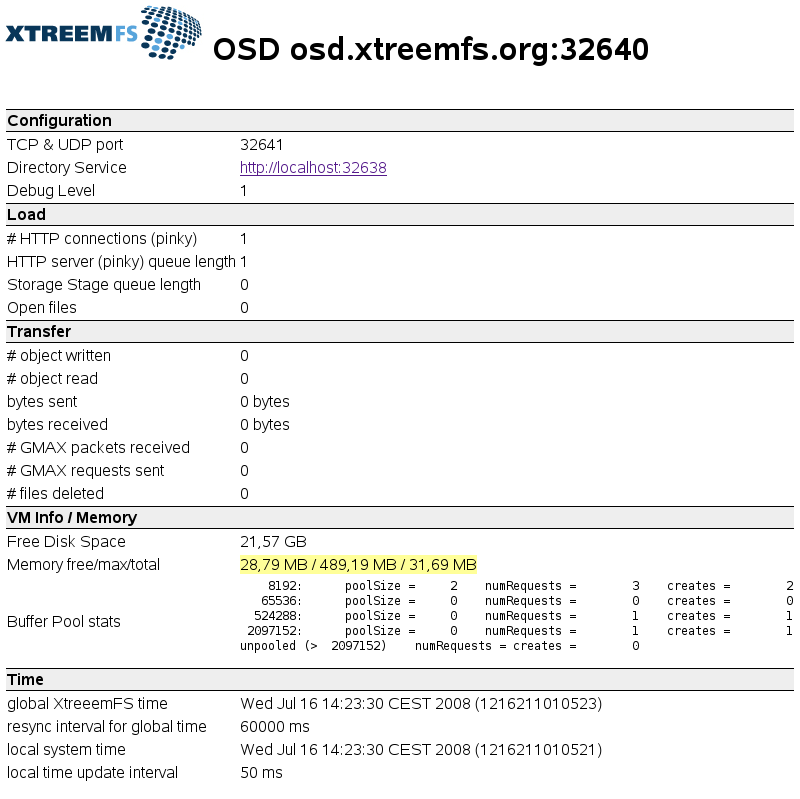
\includegraphics{images/screenshot_status.png}}
 % screenshot_status.png: 817x847 pixel, 72dpi, 28.82x29.88 cm, bb=0 0 817 847
 \caption{OSD status web page}
 \label{fig:screenshot_status}
\end{figure}

Each XtreemFS service can generate an HTML status page\index{Status Page}, which displays runtime information about the service (Fig. \ref{fig:screenshot_status}). The HTTP server that generates the status page runs on the port defined by the configuration property \texttt{http\_port}; default values are 30636 for MRCs, 30638 for Directory Services, and 30640 for OSDs.

The status page of an MRC can e.g.\ be shown by opening

\texttt{http://my-mrc-host.com:30636/}

with a common web browser. If you set an admin password in the service's configuration, you will be asked for authentication when accessing the status page. Use \texttt{admin} as user name.

\subsection{DIR Service Monitoring}

The directory service has a built-in notification system that can send alert emails if a service fails to send heartbeat messages for some time. The monitoring can be enabled in the DIR configuration by setting \texttt{monitoring = true}.

\subsection{Monitoring Services with SNMP}
\label{sec:snmpmonitoring}
All XtreemFS services can act as SNMP agent which gives the possibility to monitor status information through the SNMP protocol. To enable SNMP support for a specific service you have to set the following parameter in its configuration file: 

\begin{verbatim}
snmp.enabled = true
snmp.address = localhost
snmp.port = 34638
snmp.aclfile =  /etc/xos/xtreemfs/snmp.acl
\end{verbatim}

If \texttt{snmp.enabled} is not set to true the service will not start a SNMP agent and all other SNMP related configuration parameter will be ignored.  \texttt{snmp.port} defines the port on which the SNMP agent will listen and \texttt{snmp.address} the interface it is bound to. Since XtreemFS uses SNMPv2 which is known to be not secure it is recommended to use a dedicated monitoring network and a dedicated interface. The optional \texttt{snmp.aclfile} paramater is a path to JDMK\footnote{see \url{http://opendmk.java.net/} and \url{http://java.sun.com/products/jdmk/}} (Java Dynamic Management Kit -- the library used for providing SNMP functionality in XtreemFS) ACL file. In this file you can define who (which hosts) can use what kind of SNMP feature. Because the XtreemFS SNMP agent only provides the functionality to read values per SNMP the following example acl file is sufficient:
\begin{verbatim}
acl = {
 {
 communities = public
 access = read-only
 managers = localhost
 }
}
\end{verbatim}
\texttt{communites} is the SNMP community string your managers have to use and \texttt{managers} is a comma-separated list of hostnames, ip addresses or subnets in prefix notation (i.e. "xtreemfs-host", "192.168.0.54" or "192.168.0.3/24").

Note: If you comment out the \texttt{snmp.aclfile} line every host on your network can access all information through the SNMP agent.

If you have configured SNMP correctly an easy way to check if the SNMP agent is running is by using the \texttt{snmpget} commandline tool as follows
\begin{verbatim}
 $> snmpget -v2c -cpublic localhost:34638 1.3.6.1.4.1.38350.1.1.0 
\end{verbatim}
where "public" is the community string and the SNMP agent listens at port 9001 on localhost. "1.3.6.1.4.1.38350.1.1.0" is the OID (object identifier) which is associated with the amount of memory the JVM of this service is currently using. A list of all queryable OIDs and which information the represent can be found in the following tables.


\begin{tabular}{|l|l|l|p{5cm}|}
\hline
\multicolumn{4}{|c|}{General: These information belong to all services} \\
\hline
OID & Textual representation & Datatype & Description \\
\hline
1.3.6.1.4.1.38350.1.1.0 & jvmUsedMemory & Long &  The amount of memory that is used by the JVM this service is running into. \\
\hline
1.3.6.1.4.1.38350.1.2.0 & jvmMaxMemory & Long &  The maximum amount of memory the JVM can use. \\
\hline
1.3.6.1.4.1.38350.1.3.0 & jvmFreeMemory & Long &  The amount of free memory the JVM can still use. \\
\hline
1.3.6.1.4.1.38350.1.4.0 & rpcInterface & Integer32 &  The interface number associated with Google Protocolbuffers RPC infrastructure. \\
\hline
1.3.6.1.4.1.38350.1.5.0 & databaseVersion & String & The version of the BabuDB Database which the service is using.   \\
\hline
1.3.6.1.4.1.38350.1.6.0 & tcpPort & Integer32 &  The TCP port on which the service is listening for incomming client connections.  \\
\hline
1.3.6.1.4.1.38350.1.7.0 & debugLevel & Integer &  The current Debug Level the service has.  \\
\hline
1.3.6.1.4.1.38350.1.8.0 & numClientConnections & Integer32 & Number of active client connections. \\
\hline
1.3.6.1.4.1.38350.1.9.0 & numPendingRequests  & Long &  The number of currently pending requests. \\
\hline
1.3.6.1.4.1.38350.1.10.0 & currentTime & Long & The global time in this XtreemFS installation.  \\
\hline
1.3.6.1.4.1.38350.1.11.0 & isRunning & String & Returns whether or not the service is running. (ONLINE, OFFLINE)   \\
\hline
1.3.6.1.4.1.38350.1.12.0 & serviceType & String & Returns which kind of service this is (DIR, MRC, OSD).  \\
\hline
1.3.6.1.4.1.38350.1.13.0 & serviceUUID & String & Returns the UUID of the service. \\
\hline 
\end{tabular}

\begin{tabular}{|l|l|l|p{5cm}|}
\hline
\multicolumn{4}{|c|}{Dir: These information belong to the DIR service} \\
\hline
OID & Textual representation & Datatype & Description \\
\hline
1.3.6.1.4.1.38350.2.1.0 & addressMappingCount & Integer & The  number of address mappings currently registered at the DIR. \\
\hline
1.3.6.1.4.1.38350.2.2.0 & serviceCount & Integer & The number of services currently registered at the DIR. \\
\hline 
\end{tabular}


\begin{tabular}{|l|l|l|p{5cm}|}
\hline
\multicolumn{4}{|c|}{Mrc: These information belong to the MRC service} \\
\hline
OID & Textual representation & Datatype & Description \\
\hline
1.3.6.1.4.1.38350.3.1.0 & volumeCount & Integer &  The number of volumes currently registered at this MRC.\\
\hline
\end{tabular}

\begin{tabular}{|l|l|l|p{5cm}|}
\hline
\multicolumn{4}{|c|}{Osd: These information belong to the OSD service} \\
\hline
OID & Textual representation & Datatype & Description \\
\hline
1.3.6.1.4.1.38350.4.1.0 & numObjsRX & Long &  The number of objects this OSD has received.\\
\hline
1.3.6.1.4.1.38350.4.2.0 & numReplObjsRX & Long & The number of replicated objects this OSD has received. \\
\hline
1.3.6.1.4.1.38350.4.3.0 & numObjsTX & Long & The number of objects this OSD has transmitted. \\
\hline
1.3.6.1.4.1.38350.4.4.0 & numReplBytesRX & Long &  The number of bytes belonging to file replication this OSD has received.\\
\hline
1.3.6.1.4.1.38350.4.5.0 & numBytesRX & Long & The number of bytes this OSD has received. \\
\hline
1.3.6.1.4.1.38350.4.6.0 & numBytesTX & Long &  The number of bytes this OSD has transmitted.\\
\hline
1.3.6.1.4.1.38350.4.7.0 & preprocStageQueueLength & Integer & The current length of the preprocessing stage of this OSD. \\
\hline
1.3.6.1.4.1.38350.4.8.0 & storageStageQueueLength & Integer &  The current length of the storage stage of this OSD.\\
\hline
1.3.6.1.4.1.38350.4.9.0 & deletionStageQueueLength & Integer & The current length of the deletion stage of this OSD. \\
\hline
1.3.6.1.4.1.38350.4.10.0 & numOpenFiles & Long & The number of files this OSD has currently opened.\\
\hline
1.3.6.1.4.1.38350.4.11.0 & numDeletedFiles & Integer & The number of deleted files on this OSD. \\
\hline
1.3.6.1.4.1.38350.4.12.0 & freeSpace & Long & The free disc space on the partition this OSD stores the object files.\\
\hline
\end{tabular}

\subsection{Monitoring with Ganglia}
Ganglia\footnote{\url{http://ganglia.sourceforge.net/}} is a monitoring system specialized for environments like clusters and grids. XtreemFS provides three python based plugins for the ganglia monitoring daemon which act as SNMP manager and gather information through a local SNMP agent. 

To use these plugins you have to copy them to the \texttt{/usr/lib/ganglia/python\_modules/} directory on the host running your XtreemFS service and a ganglia monitoring daemon. You have to ensure that
\begin{enumerate}[(i)]
  \item your ganglia installation supports python modules
  \item you installed python and the pysnmp\footnote{\url{http://pysnmp.sourceforge.net/}} library which is used by the plugins
\end{enumerate}
 Also you have to configure the modules with \texttt{*.pyconf} files in the \texttt{/etc/ganglia/conf.d/} directory. I.e. to monitor a running DIR instance the following example file can be used
\newpage
\begin{verbatim}
modules {
  module {
    name = "xtfs-dir-plugin"
    language = "python"
    param Host {
      value = localhost
    }
    param Port {
      value = 34638
    }
    param CommunityString {
      value = public
    }
  }
}

collection_group {
  collect_every = 300
  time_threshold = 100
  metric {
    name = "dir_jvm_used_mem"
    title = "used memory of the jvm"
    value_threshold = 1
  }
  metric {
    name = "dir_jvm_free_mem"
    title = "free memory of the jvm"
    value_threshold = 1
  } 
  metric {
    name = "dir_client_connections"
    title = "number of Clients"
    value_threshold = 1
  }
  metric {
    name = "dir_pending_requests"
    title = "number of pending requests"
    value_threshold = 1
  }
  metric {
    name = "addr_mapping_count"
    title = "number of address mappings"
    value_threshold = 1
  }
  metric {
    name = "service_count"
    title = "number of services"
    value_threshold = 1
  }
  metric {
    name = "dir_status"
    title = "Status DIR"
  }
  metric {
    name = "dir_uuid"
    title = "DIR UUID"
  }
}
\end{verbatim}
Every XtreemFS plugin has to get 3 parameters: Host, Port, CommunityString where Host is the hostname of the SNMP agent, Port the port of the agent and CommunityString the community string as it is configured in the \texttt{snmp.acl} file. These parameters are configured in the \texttt{modules} directive. The \texttt{collection\_group} directive describes which metrics should be gathered. An overview of all possible metrics shows the \texttt{gmond -m} command. For most people the default configurations that came with your XtreemFS distribution should be sufficient. More information about ganglia, the ganglia monitoring daemon plugin system and how to configure plugins can be found at \url{http://sourceforge.net/apps/trac/ganglia}.

\section{Troubleshooting}

Various issues may occur when attempting to set up an XtreemFS server component. If a service fails to start, the log file often reveals useful information. Server log files are located in \texttt{/var/log/xtreemfs}. Note that you can restrict granularity and categories of log messages via the configuration properties \texttt{debug.level} and \texttt{debug.categories} (see Sec.\ \ref{sec:config}).

If an error occurs, please check if all of the following requirements are met:
\begin{itemize}
 \item You have root permissions when starting the service. Running the \texttt{init.d} scripts requires root permissions. However, the services themselves are started on behalf of a user \textit{xtreemfs}.
 \item DIR has been started before MRC and OSD. Problems may occur if a script starts multiple services as background processes.
 \item There are no firewall restrictions that keep XtreemFS services from communicating with each other. The default ports that need to be open are: 32636 (MRC, TCP), 32638 (DIR, TCP), and 32640 (OSD, TCP \& UDP).
 \item The MRC database version is correct. In case of an outdated database version, the \texttt{xtfs\_mrcdbtool} commands of the old and new XtreemFS version can dump and restore the database, respectively (see Sec.\ \ref{sec:mrcdbtools}).
 \item A network interface is available on the host. It may be either bound to an IPv4 or IPv6 address.
\end{itemize}


\chapter{XtreemFS Client}

The XtreemFS client is needed to access an XtreemFS installation from a local or remote machine. This chapter describes how to use the XtreemFS client in order to work with XtreemFS like a local file system.

\section{Installation}
\label{sec:client_installation}

There are two different installation sources for the XtreemFS Client: \emph{pre-packaged releases} and \emph{source tarballs}.

Note that the source tarball contains the complete distribution of XtreemFS, which also includes server and tools. Currently, binary distributions of the client are only available for Linux and Windows.

\subsection{Prerequisites}

To install XtreemFS on Linux, please make sure that FUSE 2.6 or newer, boost 1.35 or newer, openSSL 0.9.8 or newer, libattr and a Linux 2.6 kernel are available on your system. For an optimal performance, we suggest to use FUSE 2.8 with a kernel version 2.6.26 or newer.

\subsection{Installing from Pre-Packaged Releases}

On RPM-based distributions (RedHat, Fedora, SuSE, Mandriva) you can install the package with

\begin{verbatim}
$> rpm -i xtreemfs-client-1.3.x.rpm
\end{verbatim}


For Debian-based distributions, please use the \texttt{.deb} package provided and install it with

\begin{verbatim}
$> dpkg -i xtreemfs-client-1.3.x.deb
\end{verbatim}


For Windows, please use the \emph{.msi} installer that will guide you through the installation process.
For Mac OS X, we provide packaged client with installer.

\subsection{Installing from Sources}

Extract the tarball with the sources. Change to the top level directory and execute

\begin{verbatim}
$> make client
\end{verbatim}

This will build the XtreemFS client and non-Java-based tools. Note that the following third-party packages are required on Linux:

\begin{itemize}
 \item RPM-based distros: \begin{verbatim}
cmake >= 2.6
gcc-c++ >= 4.1
fuse >= 2.6
fuse-devel >= 2.6
boost-devel >= 1.35
openssl-devel >= 0.9.8
libattr-devel >= 2
\end{verbatim}

 \item DEB-based distros: \begin{verbatim}
cmake (>= 2.6)
build-essential (>=11)
libfuse-dev (>= 2.6)
libssl-dev (>= 0.9)
libattr-dev (>= 2)
libboost-system1.35-dev or later
libboost-thread1.35-dev or later
libboost-program-options1.35-dev or later
libboost-regex1.35-dev or later
\end{verbatim}
\end{itemize}

When done, execute

\begin{verbatim}
$> sudo make install-client
\end{verbatim}

to complete the installation of XtreemFS.


\section{Volume Management}

Like many other file systems, XtreemFS supports the concept of volumes. A volume can be seen as a container for files and directories with its own policy settings, e.g.\ for access control and replication. Before being able to access an XtreemFS installation, at least one volume needs to be set up. This section describes how to deal with volumes in XtreemFS.

\subsection{Creating Volumes}
\label{sec:create_volume}

Volumes can be created with the \texttt{mkfs.xtreemfs} command line utility. Please see \texttt{mkfs.xtreemfs ----help} or \texttt{man mkfs.xtreemfs} for a full list of options and usage\index{Create Volume}\index{Volume!Create}\index{mkfs.xtreemfs}.

When creating a volume, you can specify the authorization policy (see Sec. \ref{sec:access_policies}) with the option \texttt{----access-control-policy} (respectively \texttt{--a}). If not specified, POSIX permissions/ACLs will be chosen by default. Unlike most other policies, authorization policies cannot be changed afterwards.

In addition, it is possible to set a default striping policy (see Sec. \ref{sec:striping_policies}). If no per-file or per-directory default striping policy overrides the volume's default striping policy, the volume's policy is assigned to all newly created files. If no volume policy is explicitly defined when creating a volume, a RAID0 policy with a stripe size of 128kB and a width of 1 will be used as the default policy.

A volume with the default options (POSIX permission model, a stripe size of 128 kB and a stripe width of 1 (i.e.\ all stripes will reside on the same OSD)) can be created as follows:


\begin{verbatim}
$> mkfs.xtreemfs my-mrc-host.com/myVolume
\end{verbatim}

Creating a volume may require privileged access, which depends on whether an administrator password is required by the MRC. To pass an administrator password, add \texttt{----admin\_password <password>} to the \texttt{mkfs.xtreemfs} command.

For a complete list of parameters, please refer to \texttt{mkfs.xtreemfs ----help} or the \texttt{man mkfs.xtreemfs} man page.

\subsection{Deleting Volumes}

Volumes can be deleted with the \texttt{rmfs.xtreemfs} tool. Deleting a volume implies that \emph{any data, i.e.\ all files and directories on the volume are irrecoverably lost}! Please see \texttt{rmfs.xtreemfs ----help} or \texttt{man rmfs.xtreemfs} for a full list of options and usage\index{Delete Volume}\index{Volume!Delete}\index{rmfs.xtreemfs}. Please also note that \texttt{rmfs.xtreemfs} does not dispose of file contents on the OSD. To reclaim storage space occupied by the volume, it is therefore necessary to either remove all files from the volume before deleting it, or to run the cleanup tool (see Section \ref{sec:scrubber_cleanup}).

The volume \texttt{myVolume} residing on the MRC \texttt{my-mrc-host.com} (listening at the default port) can e.g.\ be deleted as follows:

\begin{verbatim}
$> rmfs.xtreemfs my-mrc-host.com/myVolume
\end{verbatim}

Volume deletion is restricted to volume owners and privileged users. Similar to \texttt{mkfs.xtreemfs}, an administrator password can be specified if required.

\subsection{Listing all Volumes}

A list of all volumes can be displayed with the \texttt{lsfs.xtreemfs} tool. All volumes hosted by the MRC \texttt{my-mrc-host.com} (listening at the default port) can be listed as follows:

\begin{verbatim}
$> lsfs.xtreemfs my-mrc-host.com
\end{verbatim}

The listing of available volumes is restricted to volume owners and privileged users. Similar to \texttt{mkfs.xtreemfs}, an administrator password can be specified if required.

\section{Accessing Volumes}
\label{sec:mount_vol}

Once a volume has been created, it needs to be mounted in order to be accessed.

\subsection{Mounting and Un-mounting}

Before mounting XtreemFS volumes on a Linux machine, please ensure that the FUSE kernel module is loaded.\index{Volume!Mount}\index{Mount}\index{mount.xtreemfs} Please check your distribution's manual to see if users must be in a special group (e.g. \texttt{trusted} in openSuSE) to be allowed to mount FUSE file systems.


\begin{verbatim}
$> su
Password:
#> modprobe fuse
#> exit
\end{verbatim}


Volumes are mounted with the \texttt{mount.xtreemfs} command:


\begin{verbatim}
$> mount.xtreemfs remote.dir.machine/myVolume /xtreemfs
\end{verbatim}


\texttt{remote.dir.machine} describes the host with the Directory Service at which the volume is registered; \texttt{myVolume} is the name of the volume to be mounted. \texttt{/xtreemfs} is the directory on the local file system to which the XtreemFS volume will be mounted. For more options, please refer to \texttt{mount.xtreemfs ----help} or \texttt{man mount.xtreemfs}.

Please be aware that the Directory Service URL needs to be provided when mounting a volume, while MRC URLs are used to create volumes.

When mounting a volume, the client will immediately go into background and won't display any error messages. Use the \texttt{-f} option to prevent the mount process from going into background and get all error messages printed to the console. Alternatively, you can execute \texttt{xtfsutil ----errors <mount point>} to print the last 20 errors for a mounted volume.

To check that a volume is mounted, use the \texttt{mount} command. It outputs a list of all mounts in the system. XtreemFS volumes are listed as \texttt{type fuse}:

\begin{verbatim}
xtreemfs@localhost/xtreemfs on /xtreemfs type fuse (...)
\end{verbatim}

Volumes are unmounted with the \texttt{umount.xtreemfs} tool\index{Volume!Un-mount}\index{Unmount}\index{umount.xtreemfs}:

\begin{verbatim}
$> umount.xtreemfs /xtreemfs
\end{verbatim}

On Mac OS X, volumes are unmounted with the regular \texttt{umount} command:
\begin{verbatim}
$> umount /xtreemfs
\end{verbatim}

\subsection{Mount Options}

Access to a FUSE mount is usually restricted to the user who mounted the volume. To allow the root user or any other user on the system to access the mounted volume, the FUSE options \texttt{-o allow\_root} and \texttt{-o allow\_other} can be used with \texttt{mount.xtreemfs}. They are, however, mutually exclusive. In order to use these options, the system administrator must create a FUSE configuration file \texttt{/etc/fuse.conf} and add a line\index{allow\_others option}\index{allow\_root option}\index{user\_allow\_other option} \texttt{user\_allow\_other}.

By default, the local system cache on the client machine will be used to speed up read access to XtreemFS. In particular, using the cache as a local buffer is necessary to support the \texttt{mmap} system call, which - amongst others - is required to execute applications on Linux. Additionally, it enables the read-ahead functionality of Fuse and does speed up sequential reads, especially in presence of high latencies. If the local system cache is not disabled, the consistency model of client caches is limited to ``close-to-open'', which is similar to the model provided by NFS. Buffered I/O can be switched off by adding the \texttt{-o direct\_io} parameter. The parameter effects that all read and write operations are directed to their OSDs instead of being served from local caches. Enabling \texttt{-o direct\_io} might be also necessary if you rely on interruption support of read requests in Linux. Please see \href{http://code.google.com/p/xtreemfs/issues/detail?id=229}{issue 229} for more details.


\section{Troubleshooting}

Different kinds of problems may occur when trying to create, mount or access files in a volume. By default errors are logged to the console. Once \texttt{mount.xtreemfs} moved into background, use \texttt{xtfsutil ----errors <mount point>} to print the last 20 errors for a mounted volume. Additionally, the tools \texttt{mkfs.xtreemfs}, \texttt{rmfs.xtreemfs}, \texttt{lsfs.xtreemfs} and \texttt{mount.xtreemfs} allow to log error messages to a logfile which has to be specified by the \texttt{--l} option. Use the \texttt{--d} option to specify the minimum severity of to be logged events.

For quickly identifying problems and testing, we recommend to run the client \texttt{mount.xtreemfs} in the foreground (option \texttt{--f}) and increase the debugging level (option \texttt{--d}). This can be done as follows:

\begin{verbatim}
$> mount.xtreemfs -f -d DEBUG remote.dir.machine/myVolume /xtreemfs
\end{verbatim}

The following list contains the most common problems and their solutions.

\begin{tabular}{lp{10cm}}
 \textbf{Problem}  & \textbf{A volume cannot be created or mounted.} \\
 \textbf{Solution} & Please check your firewall settings on the server side. Are all ports accessible? The default ports are 32636 (MRC), 32638 (DIR), and 32640 (OSD).

 In case the XtreemFS installation has been set up behind a NAT, it is possible that services registered their NAT-internal network interfaces at the DIR. In this case, clients cannot properly resolve server addresses, even if port forwarding is enabled. Please check the \emph{Address Mappings} section on the DIR status page to ensure that externally reachable network interfaces have been registered for the your servers' UUIDs. If this is not the case, it is possible to explicitly specify the network interfaces to register via the \texttt{hostname} property (see Sec.\ \ref{sec:config}).
\end{tabular}

\begin{tabular}{lp{10cm}}
 \textbf{Problem}  & \textbf{An error occurs when trying to access a mounted volume.} \\
 \textbf{Solution} & Please make sure that you have sufficient access rights to the volume root. Superusers and volume owners can change these rights via \texttt{chmod <mode> <mountpoint>}. If you try to access a mount point to which XtreemFS was mounted by a different user, please make sure that the volume is mounted with \texttt{mount.xtreemfs -o allow\_other \dots}.
\end{tabular}

\begin{tabular}{lp{10cm}}
 \textbf{Problem}  & \textbf{An I/O error occurs when trying to create new files.} \\
 \textbf{Solution} & In general, you can check the output of \texttt{xtfsutil ----errors <mount point>} to see the error which caused the I/O error. A common reason for this problem is that no OSD could be assigned to the new file. Please check if suitable OSDs are available for the volume. There are two alternative ways to do this:
   \begin{itemize}
     \item Execute \texttt{xtfsutil <mountpoint>}.
     \item Open the MRC status page. It can be accessed via \texttt{http://<MRC-host>:30636} in the default case. For each volume, a list of suitable OSDs is shown there.
   \end{itemize}
 There may be different reasons for missing suitable OSDs:
   \begin{itemize}
    \item One or more OSDs failed to start up. Please check the log files and status pages of all OSDs to ensure that they are running.
    \item One or more OSDs failed to register or regularly report activity at the DIR. Please check the DIR status page to ensure that all OSDs are registered and active.
    \item There are no OSDs with a sufficient amount of free disk space. Please check the OSD status page to obtain information about free disk space.
   \end{itemize}
\end{tabular}

\begin{tabular}{lp{10cm}}
 \textbf{Problem}  & \textbf{An I/O error occurs when trying to access an existing file.}\\
 \textbf{Solution} & Please check whether all OSDs assigned to the file are running and reachable. This can be done as follows:
    \begin{enumerate}
     \item Get the list of all OSDs for the file: \texttt{xtfsutil <file>}.
     \item Check whether the OSDs in (one of) all replicas in the list are running and reachable, e.g.\ by opening the status pages or via \texttt{telnet <host> <port>}.
    \end{enumerate}
\end{tabular}


\chapter{XtreemFS Tools}

To make use of most of the advanced XtreemFS features, XtreemFS offers a variety of tools. There are tools that support administrators with the maintenance of an XtreemFS installation, as well as tools for controlling features like replication and striping. An overview of the different tools with descriptions of how to use them are provided in the following.

\section{Installation}

The user tools are built, packaged and installed together with the XtreemFS client. For details on how to install the XtreemFS client, please refer to Section \ref{sec:client_installation}.

To install XtreemFS admin tools, you can choose from two different installation sources: you can download one of the \emph{pre-packaged releases} that we create for most Linux distributions or you can install directly from the \emph{source tarball}.

Note that the source tarball contains the complete distribution of XtreemFS, which also includes client and server. Currently, binary distributions of the admin tools are only available for Linux.

\subsection{Prerequisites}

For the pre-packaged release, you will need Sun Java JRE 1.6.0 or newer to be installed on the system. Some tools also require the \texttt{attr}/\texttt{libattr} package to be installed.

When building XtreemFS directly from the source, you need a Sun Java JDK 1.6.0 or newer, Ant 1.6.5 or newer and gmake.

\subsection{Installing from Pre-Packaged Releases}

On RPM-based distributions (RedHat, Fedora, SuSE, Mandriva) you can install the package with

\begin{verbatim}
$> rpm -i xtreemfs-tools-1.3.x.rpm xtreemfs-backend-1.3.x.rpm
\end{verbatim}


For Debian-based distributions, please use the \texttt{.deb} package provided and install it with

\begin{verbatim}
$> dpkg -i xtreemfs-tools-1.3.x.deb xtreemfs-backend-1.3.x.deb
\end{verbatim}

To install the tools, the following package is required: \texttt{jre} $\geq$ 1.6.0 for RPM-based releases, \texttt{java6-runtime} for Debian-based releases. If you already have a different distribution of \texttt{Java6} on your system, you can alternatively install the XtreemFS tools packages as follows:

\begin{verbatim}
$> rpm -i --nodeps xtreemfs-tools-1.3.x.rpm \
   xtreemfs-backend-1.3.x.rpm
\end{verbatim}

on RPM-based distributions,

\begin{verbatim}
$> dpkg -i --ignore-depends java6-runtime \
   xtreemfs-tools-1.3.x.deb xtreemfs-backend-1.3.x.deb
\end{verbatim}

on Debian-based distributions.

To ensure that your local \texttt{Java6} installation is used, is necessary to set the \texttt{JAVA\_HOME} environment variable to your \texttt{Java6} installation directory, e.g.\

\begin{verbatim}
$> export JAVA_HOME=/usr/java6
\end{verbatim}


All XtreemFS tools will be installed to \texttt{/usr/bin}.

\subsection{Installing from Sources}

Extract the tarball with the sources. Change to the top level directory and execute

\begin{verbatim}
$> make server
\end{verbatim}

When done, execute

\begin{verbatim}
$> sudo make install-tools
\end{verbatim}

to complete the installation. Note that this will also install the XtreemFS client and servers.

\section{Admin Tools}

This section describes the tools that support administrators in maintaining an XtreemFS installation.

\subsection{MRC Database Conversion}
\label{sec:mrcdbtools}

The database format in which the MRC stores its file system metadata on disk may change with future XtreemFS versions, even though we attempt to keep it as stable as possible. To ensure that XtreemFS server components may be updated without having to create and restore a backup of the entire installation, it is possible to convert an MRC database to a newer version by means of a version-independent XML representation.

This is done as follows:
\begin{enumerate}
  \item Create an XML representation of the old database with the old MRC version.
  \item Update the MRC to the new version.
  \item Restore the database from the XML representation.
\end{enumerate}

\texttt{xtfs\_mrcdbtool} is a tool that is capable of doing this. It can create an XML dump of an MRC database as follows:

\begin{verbatim}
$> xtfs_mrcdbtool -mrc pbrpc://my-mrc-host.com:32636 \
   dump /tmp/dump.xml
\end{verbatim}

A file \texttt{dump.xml} containing the entire database content of the MRC running on \texttt{my-mrc-host.com:32636} is written to \texttt{/tmp/dump.xml}. For security reasons, the dump file will be created locally on the MRC host. To make sure that sufficient write permissions are granted to create the dump file, we therefore recommend to specify an absolute dump file path like \texttt{/tmp/dump.xml}.

A database dump can be restored from a dump file as follows:

\begin{verbatim}
$> xtfs_mrcdbtool -mrc pbrpc://my-mrc-host.com:32636 \
   restore /tmp/dump.xml
\end{verbatim}

This will restore the database stored in \texttt{/tmp/dump.xml} at \texttt{my-mrc-host.com}. Note that for safety reasons, it is only possible to restore a database from a dump if the database of the running MRC does not have any content. To restore an MRC database, it is thus necessary to delete all MRC database files before starting the MRC.

Please be aware that dumping and restoring databases may both require privileged access rights if the MRC requires an administrator password. The password can be specified via \texttt{----admin\_password}; for further details, check the \texttt{xtfs\_mrcdbtool} man page.

\subsection{Scrubbing and Cleanup}
\label{sec:scrubber_cleanup}

In real-world environments, errors occur in the course of creating, modifying or deleting files. This can cause corruptions of file data or metadata. Such things happen e.g.\ if the client is suddenly terminated, or loses connection with a server component. There are several such scenarios: if a client writes to a file but does not report file sizes received from the OSD back to the MRC, inconsistencies between the file size stored in the MRC and the actual size of all objects in the OSD will occur. If a client deletes a file from the directory tree, but cannot reach the OSD, orphaned objects will remain on the OSD. If an OSD is terminated during an ongoing write operation, file content will become corrupted.

In order to detect and, if possible, resolve such inconsistencies, tools for scrubbing and OSD cleanup exist. To check the consistency of file sizes and checksums, the following command can be executed:

\begin{verbatim}
$> xtfs_scrub -dir pbrpc://my-dir-host.com:32638 myVolume
\end{verbatim}

This will scrub each file in the volume \texttt{myVolume}, i.e.\ check file size consistency and set the correct file size on the MRC, if necessary, and check whether an invalid checksum in the OSD indicates a corrupted file content. The \texttt{-dir} argument specifies the directory service that will be used to resolve service UUIDs. Please see \texttt{man xtfs\_scrub} for further details.

A second tool scans an OSD for orphaned objects, which can be used as follows:

\begin{verbatim}
$> xtfs_cleanup -dir pbrpc://localhost:32638 \
   uuid:u2i3-28isu2-iwuv29-isjd83
\end{verbatim}
The given UUID identifies the OSD to clean and will be resolved by the
directory service defined by the \texttt{-dir} option (localhost:32638 in this example).
The process will be started and can be stopped by setting the option
\texttt{-stop}. To watch the cleanup progress use option \texttt{-i} for the
interactive mode. For further information see \texttt{man xtfs\_cleanup}.

\subsection{Setting the Service Status}

The service's status field is shown in the service status page as \texttt{static.status}. The status can be 0 (online), 1 (marked for removal) and 2 (dead/removed). Status 0 (online) is the regular status for all services, even if they are temporarily offline. Status 2 (dead/removed) marks an OSD as permanently failed and the scrubber will removed replicas and files from these OSDs. Status 1 (marked for removal) is for future use.

The status can be set with the \texttt{xtfs\_chstatus} tool:

\begin{verbatim}
$> xtfs_chstatus -dir pbrpc://localhost:32638 \
   u2i3-28isu2-iwuv29-isjd83 online
\end{verbatim}

This command sets the status of the service with the UUID \texttt{u2i3-28isu2-iwuv29-isjd83} to online.

% \subsection{Drain an OSD}
% To drain a running OSD from the system all object files stored on this OSD have to be moved to another one. This can be done with the \texttt{tunefs do} (\texttt{tunefs drainosd} for the long version) command. The syntax is in the following way:
% 
% \begin{verbatim}
% $> tunefs.xtreemfs --dir pbrpc://<hostname|IP address>:<port>\
%    do <UUID of an OSD>
% \end{verbatim}
% 
% You have to consider that this command needs explicitly the address of the DIR service provided by the \texttt{---dir} option. Furthermore if you have configured an administrator password for the DIR service this has to be specified with the \texttt{---password} or \texttt{-p} option, otherwise the OSD can't be shutdown and this step has to be done manually. An example for shutting down an OSD with the UUID \linebreak \texttt{u2i3-28isu2-iwuv29-isjd83} looks like as follows:
% 
% \begin{verbatim}
% $> tunefs.xtreemfs --dir pbrpc://localhost:32638  \
%    -p mySecretPass do u2i3-28isu2-iwuv29-isjd83
% \end{verbatim}
% 
% Internally the \texttt{tunefs do} command works by using the read-only replication feature. All files of which an OSD has got object files will be set to read-only. Afterwards for these files a new replica will be created and the replication triggered. When the replication is completed all the original replicas will be removed and the OSD shut down. If an error occurs while doing these steps all changes to files will be reverted.
% 
% Note that these steps are done mostly on client side to avoid to much load on other services. Therefore the execution time of this command can be very high, especially when dealing with a large amount of files. 

\subsection{Snapshots}

XtreemFS is capable of taking file system snapshots. A snapshot captures an instantaneous image of all files and directories in a volume, which can later be accessed in a read-only manner.

Snapshots can be created, listed and deleted with the \texttt{xtfs\_snap} tool. A mounted volume is necessary to run the tool; information on how to mount volumes can be found in Section \ref{sec:mount_vol}.

As snapshots cause an additional storage and I/O overhead since they require copy-on-write versioning of files across the OSDs, it is first necessary to enable them on a volume. Snapshots can be enabled as follows:

\begin{verbatim}
$> xtfs_snap --enable -d /path/to/mounted/volume
\end{verbatim}

Once snapshots have been enabled, a snapshot named \texttt{mySnapshot} can be taken as follows:

\begin{verbatim}
$> xtfs_snap -c -r -d /path/to/mounted/volume/subdirectory \
   mySnapshot
\end{verbatim}

The optional \texttt{-r} parameter enables a recursive capturing that includes all subdirectories beneath the XtreemFS directory \texttt{subdirectory}.

A list of all snapshots that exist on the volume can be displayed as follows:

\begin{verbatim}
$> xtfs_snap -l -d /path/to/mounted/volume
mySnapshot
\end{verbatim}

Snapshots are exposed as read-only volumes. To access a snapshot, it is necessary to mount it. The volume name is composed of the original volume name and the snapshot name, separated by an \texttt{@} character. Mounting a snapshot works as follows:

\begin{verbatim}
$> mount.xtreemfs localhost/volume@mySnapshot \
   /path/to/mounted/volume2
\end{verbatim}

A mounted volume snapshot can be browsed normally, and all files can be read as on the original volume. However, any attempt to write data on a snapshot will result in an \texttt{EPERM} error.

A snapshot \texttt{mySnapshot} that is no longer needed can be removed as follows:

\begin{verbatim}
$> xtfs_snap -x -d /path/to/mounted/volume mySnapshot
\end{verbatim}

Please be aware that removing a snapshot does not automatically reclaim storage space from all prior versions. To dispose of obsolete and redundant versions on a specific OSD, it is necessary to perform a version cleanup run with the \texttt{xtfs\_cleanup} tool:

\begin{verbatim}
$> xtfs_cleanup -dir localhost:32638 -v \
   uuid:8bca70da-c963-43c7-b30b-d0d605d39fa7
\end{verbatim}

\textbf{Note:} A snapshot only captures a file in its current state if it is \emph{closed}. Files that are \emph{open} when taking a snapshot are captured in the last state in which they were before they were opened. Since files are implicitly closed on an OSD through a timeout rather than an explicit \texttt{close} call, it may happen that files are not included in a snapshot despite having been closed at application level before the snapshot was taken. To make sure a change to a specific file is included in a subsequent snapshot, it is necessary to wait for the close timeout on the OSD before taking the snapshot, which by default is set to 60 seconds.

\subsection{Draining OSDs}

In some cases, it may be necessary to remove an OSD from an XtreemFS installation. The OSD drain tool removes an OSD without losing the files stored on it. This is done by distributing the files across the remaining OSDs before performing the removal. The tool can be used as follows:

\begin{verbatim}
$> xtfs_remove_osd -dir localhost:32638 \
   uuid:8bca70da-c963-43c7-b30b-d0d605d39fa7
\end{verbatim}

Executing the command will drain the OSD with the given UUID that was registered at the given DIR. A drained OSD will not be assigned to new files. By default, it will remain in the system until it is manually shut down by the administrator. To perform an automatic shutdown, use the \texttt{-s} switch. Please refer to the man page for further details.

\subsubsection{How it Works}

Draining an OSD works as follows:
\begin{enumerate}
 \item The OSD is marked as ``locked''. This restrains it from being assigned to newly created files.
 \item A new replica is added to each file stored on the OSD. The OSD used for this replica is selected according to the volume's OSD selection policy (see Section \ref{sec:osd_policies}).
 \item Once the new replica has become consistent, i.e. all content has been copied from the original replica, the original replica (which is stored on the OSD that is supposed to be drained) is removed.
 \item As soon as all replicas have been removed, the draining procedure has finished. 
\end{enumerate}

\subsubsection{Limitations}

While the draining is in progress, it is not possible to modify the to be moved files as they are temporarily set to read-only. Additionally, when the draining will be started, no files of the OSD should be hold open by any client.

Draining an OSD that holds striped and replicated files involves certain limitations. A striped file is currently moved to a new OSD in its entirety rather than partially. Regardless of the original number of OSDs it was striped across, it is relocated to a single target OSD, which implies that the target file is not striped anymore. As a consequence, data may be moved from OSDs that are not directly affected by the draining process.

Furthermore, at least one OSD has to exist for each file that does not hold any data of the file, i.e.\ is not included in any stripe or replica. If all OSDs that are eligible according to the OSD selection policy have already been assigned to a file, draining any of these OSDs will fail, as no additional replicas can be created.

\section{User Tools}

Since release 1.3, all user tools have been replaced by the \texttt{xtfsutil} tool. \texttt{xtfsutil} displays XtreemFS specific file and directory information, manages file replicas and volume policies.

\subsection{\texttt{xtfsutil} for Files}
\label{sec:xtfsutil_files}

When called without any option \texttt{xtfsutil} prints the XtreemFS specific information for a volume, directory, softlink or file.

\begin{verbatim}
$> cd /xtreemfs
$> echo 'Hello World' > test.txt
$> xtfsutil test.txt
\end{verbatim}


will produce output similar to the following:

\begin{verbatim}
Path (on volume)     /test.txt
XtreemFS file Id     1089e4fb-9eb9-46ea-8acf-91d10c2170e3:2
XtreemFS URL         pbrpc://localhost:32638/xtreemfs/test.txt
Owner                user
Group                users
Type                 file
Replication policy   WqRq
XLoc version         0
Replicas:
  Replica 1
     Striping policy     STRIPING_POLICY_RAID0 / 1 / 128kB
     Replication Flags   partial
     OSD 1               test-osd1/127.0.0.1:32641
  Replica 2
     Striping policy     STRIPING_POLICY_RAID0 / 1 / 128kB
     Replication Flags   partial
     OSD 1               test-osd0/127.0.0.1:32640
  Replica 3
     Striping policy     STRIPING_POLICY_RAID0 / 1 / 128kB
     Replication Flags   partial
     OSD 1               test-osd2/127.0.0.1:32642
\end{verbatim}


The fileID\index{fileID} is the unique identifier within XtreemFS, e.g. used by the OSD to identify the file's objects. The owner/group fields are shown as reported by the MRC, you may see other names on your local system if there is no mapping (i.e.\ the file owner does not exist as a user on your local machine). The XtreemFS URL shows you on which MRC the volume is hosted and the name of the volume. This file has three replicas and is replicated with the \texttt{WqRq} policy (majority voting).

\subsubsection{Changing the Replication Policy}

The replication policy defines how a file is replicated. The policy can only be changed for a file that has no replicas. If you wish to change the policy for a replicated file, you have to remove all replicas first.

To change the replication policy, execute \texttt{xtfsutil} with the following options:

\begin{verbatim}
$> xtfsutil --set-replication-policy ronly /xtreemfs/test.txt
\end{verbatim}

The following values (or its aliases stated in parentheses) can be passed to \verb|--set-replication-policy|:
\begin{description}
  \item[none] File is not replicated.
  \item[ronly (readonly)] File is read-only replicated and will be marked as read-only, i.e. the file cannot be modified as long as the replication policy is set to \textbf{ronly}.
  \item[WqRq (quorum), WaR1 (all)] The file will be read-write replicated and can be modified. Please refer to the Section \ref{sec:readwrite_replication} for more information on both policies and their properties.
\end{description}


\subsubsection{Adding and Removing Replicas}

Replicas can be added for files that have a replication policy defined, i.e. not \texttt{none}. When adding a replica, you need to specify on which OSD to create the new replica. Alternatively, you can use \texttt{AUTO} instead of an OSD UUID. With \texttt{AUTO} set, the \texttt{xtfsutil} will automatically select an OSD.

To add a replica execute:

\begin{verbatim}
$> xtfsutil --add-replica AUTO /xtreemfs/test.txt
\end{verbatim}

For read-only replicated files, replicas are partial by default. To create a full replica, you can use the \verb|--full| flag when adding a replica. For read-write replicated files, all replicas are equal and there is no further options.

In case you want to select an OSD for a new replica manually, you can retrieve a list of up to 10 OSDs for a file. The MRC automatically filters and sorts the list of OSDs depending on the policies set for a volume. In addition, the MRC also excludes all OSDs that already have a replica of that file. To retrieve this list execute:

\begin{verbatim}
$> xtfsutil --list-osds /xtreemfs/test.txt
OSDs suitable for new replicas: 
  test-osd1
  test-osd2
\end{verbatim}

To remove a replica, pass the OSD's UUID to \texttt{xtfsutil}:

\begin{verbatim}
$> xtfsutil --delete-replica test-osd1 /xtreemfs/test.txt
\end{verbatim}

\subsection{\texttt{xtfsutil} for Volumes}
\label{sec:xtfsutil_volumes}

To display the volume policies and settings, execute \texttt{xtfsutil} on the mountpoint without any options.

\begin{verbatim}
$> xtfsutil /xtreemfs
\end{verbatim}

will produce output similar to the following:

\begin{verbatim}
Path (on volume)     /
XtreemFS file Id     1089e4fb-9eb9-46ea-8acf-91d10c2170e3:1
XtreemFS URL         pbrpc://localhost:32638/replicated
Owner                user
Group                users
Type                 volume
Free/Used Space      24 GB / 6 bytes
Num. Files/Dirs      1 / 1
Access Control p.    2
OSD Selection p.     1000,3002
Replica Selection p. default
Default Striping p.  STRIPING_POLICY_RAID0 / 1 / 128kB
Default Repl. p.     WqRq with 3 replicas
\end{verbatim}


\subsubsection{Changing the Default Striping Policies}

Currently, it is not possible to change the striping policy of an existing file, as this would require rearrangements and transfers of data between OSDs. However, it is possible to define individual striping policies for files that will be created in the future. This can be done by changing the default striping policy of the parent directory or volume.

The striping policy can be changed with \texttt{xtfsutil} as follows:

\begin{verbatim}
$> xtfsutil --set-dsp -p RAID0 -w 4 -s 256 /xtreemfs
\end{verbatim}

This will cause a RAID0 striping policy with 256kB stripe size and four OSDs to be assigned to all newly created files in \texttt{/xtreemfs}.

When creating a new file, XtreemFS will first check whether a default striping policy has been assigned to the file's parent directory. If this is not the case, the default striping policy for the volume will be used as the striping policy for the new file. Changing a volume's or directory's default striping policy requires superuser access rights, or ownership of the volume or directory.


\subsubsection{Changing the Default Replication Policy}

The Default Replication Policy defines how new files on a volume are replicated. This policy can be set on the volume and is valid for all sub-directories. It affects only new files and doesn't modify the replication settings for existing files.

The replication policy can be changed as follows. In this example, all files will have three replicas with WqRq mode.
\begin{verbatim}
$> xtfsutil --set-drp --replication-policy WqRq \
            --replication-factor 3 /xtreemfs
\end{verbatim}

The following values (or its aliases stated in parentheses) can be passed to \verb|--replication-policy|:
\begin{description}
  \item[none] New files are not replicated.
  \item[ronly (readonly)] Files are initially created without replicas and can be modified until they are closed. On close, the file is set to read-only and the replicas are created. Replicas are partial by default. Full replicas will be created if the \verb|--full| flag is set.
  \item[WqRq (quorum), WaR1 (all)] New files are read-write replicated and can be modified. Please refer to the Section \ref{sec:readwrite_replication} for more information on both policies and their properties.
\end{description}


\subsection{Changing OSD and Replica Selection Policies}\label{sec:osd_select_policy}

When creating a new file, OSDs have to be selected on which to store the file content. Likewise, OSDs have to be selected for a newly added replica, as well as the order in which replicas are contacted when accessing a file. How these selections are done can be controlled by the user.

OSD and replica selection policies can only be set for the entire volume. Further details about the policies are described in Sec.\ \ref{sec:osd_policies}.

The policies are set and modified with the \texttt{xtfsutil} tool on the volume (mount point). When called without any options, \texttt{xtfsutil} will also show the policies currently set for the volume. A policy that controls the selection of a replica is set as follows:

\begin{verbatim}
 $> xtfsutil --set-rsp dcmap /xtreemfs
\end{verbatim}

This will change the current replica selection policy to a policy based on a data center map.

Note that by default, there is no replica selection policy, which means that the client will attempt to access replicas in their natural order, i.e.\ the order in which the replicas have been created.

Similar to replica selection policies, OSD selection policies are set and retrieved:

\begin{verbatim}
 $> xtfsutil --set-osp dcmap /xtreemfs
\end{verbatim}

sets a data center map-based OSD selection policy, which is invoked each time a new file or replica is created. The following predefined policies exist (see Sec.\ \ref{sec:osd_policies} and \texttt{man xtfsutil} for details):

\begin{description}
 \item[\texttt{default}] The default OSD selection policy selects a random subset of OSDs that are responsive and have more than 2GB of free disk space.
 \item[\texttt{fqdn}] Selects OSDs based on the size of the post-fix match of the fully qualified domain names and on the free space.
 \item[\texttt{dcmap}] Selects OSDs based on the distance defined in the datacenter map and on the free space.
 \item[\texttt{vivaldi}] Selects OSDs based on the distance of the Vivaldi coordinates between client and OSD and on the free space.
\end{description}

In addition, custom policies can be set by passing a list of basic policy IDs to be successively applied instead of a predefined policy name.


\subsection{Setting and Listing Policy Attributes}
\label{sec:policyAttributes}

OSD and replica selection policy behavior can be further specified by means of policy attributes.

An individual attribute for a policy (see Section \ref{sec:predefinedPolicies}) can be defined by using a combined key consisting of policy ID to the attriubte name, e.g.:

\begin{verbatim}
 $> xtfsutil --set-pattr 1001.domains \
    --value "*.xtreemfs.org bla.com" /xtreemfs
\end{verbatim}

Policy attributes can be removed by setting an empty value, e.g.:

\begin{verbatim}
 $> xtfsutil --set-pattr 1001.domains --value "" /xtreemfs
\end{verbatim}

A list of all policy attributes that have been set can be shown as follows:

\begin{verbatim}
 $> xtfsutil --list-pattrs /xtreemfs
\end{verbatim}

Please note that it is no longer possible to specify global policy attributes without a specific policy ID.

\subsection{Modifying Access Control Lists}

In some cases, it may be necessary to enforce access control on a file or directory at a finer granularity than expressible with simple ``rwx''-like access rights. XtreemFS supports Access Control Lists (ACLs) to set individual access rights for users and groups.

An ACL entry for the user \texttt{someone} with the value \texttt{rx} (``read or execute'') can be added as follows:

\begin{verbatim}
 $> xtfsutil --set-acl u:someone:rx /xtreemfs
\end{verbatim}

An existing entry can be removed as follows:

\begin{verbatim}
 $> xtfsutil --del-acl u:someone /xtreemfs
\end{verbatim}

Please be aware that when files or directories are accessed, the actual evaluation of ACL entries depends upon the effective authorization policy on the volume (see Section \ref{sec:access_policies}). With a POSIX authorization policy, ACL entries will be evaluated as described at \href{http://www.suse.de/~agruen/acl/linux-acls/online}{http://www.suse.de/\~{}agruen/acl/linux-acls/online}.

\section{Vivaldi}
\label{sec:vivaldi}
\textbf{Attention:} Vivaldi is currently not included in Release 1.3.x but will become available in one of the next major releases.
Client machines that want to use vivaldi network coordinates for replica and OSD selection must calculate their own coordinates relative to the OSDs. This is done by the \texttt{xtfs\_vivaldi} utility which must be started on each client machine. Ideally, this process is started during boot with the \texttt{xtreemfs-vivaldi} init.d scripts provided. The utility must be started with the directory service address and the path to a file in which the coordinates are stored.

\begin{verbatim}
 $> xtfs_vivaldi remote.dir.machine \
    /var/lib/xtreemfs/vivaldi_coordinates
\end{verbatim}

If started with the init.d script, the utility will get the DIR address from\\ \texttt{/etc/xos/xtreemfs/default\_dir} and will store the coordinates in\\ \texttt{/var/lib/xtreemfs/vivaldi\_coordinates}.

The coordinate file must be passed as an argument when mounting a volume:

\begin{verbatim}
$> mount.xtreemfs --vivaldi-coordinates-file-path \
   /var/lib/xtreemfs/vivaldi_coordinates \
   remote.dir.machine/myVolume /xtreemfs
\end{verbatim}

Finally, the vivaldi replica and OSD selection policies must be set at the MRC for the volume(s). See Sec. \ref{sec:osd_select_policy} for details.

\section{Test Tools}
XtreemFS provides two tools to simplify testing. \texttt{xstartserv} can be used to start and stop XtreemFS servers manually. \texttt{xtestenv} automatically sets-up an entire test environment with servers and mounted clients. In addition, \texttt{xtestenv} can be used to execute the automatic integration tests.

\chapter{Replication}

XtreemFS offers replication of all data. On the one hand, the Directory Service (DIR) and the Metadata Catalog (MRC) are replicated at database level. On the other hand, files are replicated on the OSDs with read/write or with read-only replication. In this chapter, we describe how these replication mechanisms work, their requirements and potential use-cases.

\section{Read/Write File Replication}
\label{sec:readwrite_replication}
File that are replicated with read/write replication have the same semantics as non-replicated files. That means that all operations can be executed on those files and that data is kept consistent across replicas. Applications and users won't see a difference between read/write replicated and regular files.

\subsection{Technical Details}
Internally, the read/write replication is implemented using the primary/backup approach with leases. When a file is opened, all OSDs that have a replica ``talk'' to each other to decide which replica becomes the \textit{primary}. In XtreemFS we use leases for the primary election, this means that an OSD will become primary for some time. As long as the file is accessed on the OSD, the lease will be periodically renewed in the background. If the OSD fails, the lease times out and another OSD can become primary.
Once a replica has acquired the lease to become primary, it checks with the other replicas to ensure all replicas are in a consistent state. After this so called replica reset phase, the primary processes client operations.
Reads can be executed locally on the primary. However, operations that modify data such as write and truncate, are executed on the primary which passes these updates on to the other replicas (backups).

The replication of files adds significant communication overhead to keep replicas in sync. When a file is opened, the OSD which the client contacts requires at least three message round-trips to acquire the lease and to execute the replica reset. Once a primary was elected, read operations can be executed locally without any communication. Truncate and write require a single round-trip between the primary and the backup OSDs.

Depending on the selected replication policy, the read/write replication can tolerate some replica failures. The \textbf{WqRq} (\textit{write quorum, read quorum}) policy employs majority voting and can tolerate replica failures as long as a majority of replicas is available. This is the most fault-tolerant strategy in XtreemFS. However, it guarantees only that data is stored on a majority of the replicas. If you lose more replicas permanently, data might be lost. Please note that, unlike the term \textit{read quorum} suggests, read operations are not executed on the majority of replicas. Instead it means that a majority of replicas has to be available during the replica reset phase in order to synchronize the primary's replica. After this phase read operations are executed locally. Please keep in mind that the majority of two replicas is two, i.e. using WqRq with two replicas will provide you no availability in case of a replica failure. Use the WqRq policy only if you have at least 3 OSDs - otherwise select the WqR1 policy.

The \textbf{WaR1} (\textit{write all, read 1}) policy writes updates to all replicas which yields higher data safety. However, if any replica is unavailable, modifications are not possible and the client will receive a write error. Local data can be still read from an OSD.

\subsection{Limitations}
Due to the communication overhead, the read/write replication should only be used for up to ten replicas. If you need more replicas or if you need replicas for caching, you should consider the read-only replication.

\subsection{Setup}
To enable read/write replication, it is necessary to specify a respective replication policy. Replication policies that enable read/write replication are \textbf{WqRq} and \textbf{WaR1}.

A replication policy can either be specified for an existing file or as a default policy for the entire volume. In the former case, replicas need to be added manually. In the latter case, a default replication factor needs to be specified that defines the number of replicas that are initially created. Please be aware that a default replication policy only affects newly created files, i.e.\ does not automatically add replicas to existing files!

For details on how to define replication policies, please refer to Section \ref{sec:xtfsutil_files} and \ref{sec:xtfsutil_volumes}.

\section{Read-Only File Replication}
\label{sec:ronly_replication}
The read-only is designed for use-cases where you have many replicas that are not modified. Since files cannot be changed, the replicas don't need to be coordinated. Therefore, this replication mode can handle as many replicas as you like, e.g. to create copies of files close to consumers. One use-case for the read-only replication is to build a content-distribution network (CDN) like infrastructure.

Read-only replicas are either \textit{full} or \textit{partial}. Full replicas immediately copy the file data from other replicas when they are created. XtreemFS uses a rarest-first strategy (similar to BitTorrent) to increase the replication factor as quickly as possible. In contrast, partial replicas are initially empty and fetch the file data (objects) on demand when requested by a client. Partial replicas also pre-fetch a small number of objects to reduce latency for further client reads.

\subsection{Limitations}
Files that are read-only replicated can only be opened in read-only mode and cannot be modified. To allow existing applications to take advantage of the read-only replication without modifications, XtreemFS offers ``replicate-on-close''. When the default replication policy for a volume is set to ``ronly'', files can be opened and modified like regular files until they are closed. Once a file is closed, it is set to read-only and is replicated according to the replication factor set for the volume. This mode should, however, not be used for data safety as there are no guarantees that all replicas were created successfully when the \texttt{close()} operation returns. For data safety, please use read/write replication.

\subsection{Setup}
Similar as with read/write replication, enabling read-only replication requires a read-only replication policy to be set. The respective policy name is \textbf{ronly}. It can either be specified for an existing file or as a default policy for the entire volume. For details on how to define replication policies, please refer to Section \ref{sec:xtfsutil_files} and \ref{sec:xtfsutil_volumes}.


\section{MRC and DIR Replication}
Aside from file replication across OSDs, XtreemFS also supports MRC and DIR replication to increase data safety. MRC replication covers all file system metadata, whereas DIR replication covers configuration information of services as well as volumes.

\subsection{Technical Details}
DIR and MRC replication rely on the same principle as read-write replication of files. A primary replica, which is distinguished by means of a lease, accepts all updates and disseminates these to all backup replicas in the same order. When the primary fails, the lease will eventually expire and one of the former backup replicas can become primary. Unlike file replication, which may involve a different set of OSDs for each file, an MRC or DIR replicates its entire database.

\subsection{Setup}
To enable database replication across a set of DIR or MRC instances, it is necessary to enable replication and configure its parameters. This needs to be done prior to starting up the services. The basic steps are the following:

\begin{itemize}
 \item Enable the replication plug-in on all replicated MRC/DIR instances
 \item Configure replication parameters across all instances
 \item Start up all replicated MRC/DIR instances
\end{itemize}

\subsubsection{Enabling and Configuring MRC Replication}
A replicated MRC consists of at least two individual server instances. Note that you will need three or more instances to be able to transparently recover from failures, as a majority of replicas always needs to be available to make progress.

To configure multiple MRC instances as replicas of each other, it is necessary to enable and configure the replication plug-in across these instances. This is done by setting the property \texttt{babudb.plugin.0} in the configuration file of each MRC instance, such that it points to the plug-in's configuration file. If the \texttt{xtreemfs-server} package has been installed, a default configuration file for the replication plug-in can be found at \texttt{/etc/xos/xtreemfs/server-repl-plugin/mrc.properties}. In order to activate the plug-in, open \texttt{/etc/xos/xtreemfs/mrcconfig.properties} with a text editor and enter (or un-comment) the following line:

\begin{verbatim}
babudb.plugin.0 = /etc/xos/xtreemfs/server-repl-plugin/mrc.properties
\end{verbatim}

Now, it is necessary to configure the replication plug-in. For this purpose, open \texttt{/etc/xos/xtreemfs/server-repl-plugin/mrc.properties} with a text editor. The configuration file will look as follows:

\begin{verbatim}
# number of servers that at least have to be up to date
babudb.repl.sync.n = 2

...

# participants of the replication including the local address
# (may be missing, if localhost was defined explicitly)
babudb.repl.participant.0 = localhost
babudb.repl.participant.0.port = 35676
babudb.repl.participant.1 = somehost
babudb.repl.participant.1.port = 35676

...
\end{verbatim}

\texttt{babudb.repl.sync.n} defines the number of servers that need to respond to an update before acknowledging the update to the client. To ensure data safety in the face of failures, it is necessary to set the property to a number that reflects at least a majority of all replicas. The list of replicas can be extended arbitrarily by adding new \texttt{babudb.repl.participant.n} as well as \texttt{babudb.repl.participant.n.port} properties, where \texttt{n} defines the replica number. Host names have to be resolvable, and hosts have to be able to reach each other on the respective ports. Please also make sure that replica lists are equivalent across all replicated MRC instances, i.e.\ each can reach all other hosts in the replica set.

Note that it is necessary to explicitly enable SSL if server-to-server authentication and encryption between replicas are required, regardless of whether an SSL-based XtreemFS installation was set up. This is because BabuDB establishes its own connection to exchange data with other replicated instances.

Please make sure that all replicated instances have consistent configurations before starting them up, which includes replica lists, \texttt{babudb.repl.sync.n} parameters as well as SSL settings if necessary.

\subsubsection{Enabling and Configuring DIR Replication}
DIR replication is enabled and configured in the exact same way as MRC replication. Change \texttt{/etc/xos/xtreemfs/server-repl-plugin/dir.properties} accordingly to configure the plug-in. In contrast to MRC replication, however, the XtreemFS client does not yet support an automatic fail-over if the DIR is not reachable.

\subsubsection{Startup and Access}
Once all service instances have been configured, they can be started up individually as described in Section \ref{sec:startstopservice}. From a user's point of view, a replicated MRC behaves exactly like a non-replicated MRC. Failures will be transparently handled by the system and hidden from users to the best possible extent. For the service to remain operable, however, at least a majority of all replicas in the list have to be reachable.


\chapter{Policies} \label{chap:policies}
Many facets of the behavior of XtreemFS can be configured by means of policies. A policy defines how a certain task is performed, e.g.\ how the MRC selects a set of OSDs for a new file, or how it distinguishes between an authorized and an unauthorized user when files are accessed. Policies are a means to customize an XtreemFS installation.

XtreemFS supports a range of predefined policies for different tasks. Alternatively, administrators may define their own policies in order to adapt XtreemFS to customer demands. This chapter contains information about predefined policies, as well as mechanisms to implement and plug in custom policies.

\section{Authentication Policies} \label{sec:authentication_policies}
Any operation on a file system is executed on behalf of a user. The process of determining the user bound to a request is generally referred to as \emph{user authentication}. To render user authentication customizable, the MRC allows administrators to specify an authentication policy by means of an \emph{Authentication Provider}\index{Authentication Provider}. Authentication Providers are modules that implement different methods for retrieving user and group IDs from requests.

The following predefined authentication providers exist:

\subsection{UNIX uid/gid - NullAuthProvider}

The NullAuthProvider\index{Authentication Provider!NullAuthProvider}\index{NullAuthProvider} is the default Authentication Provider. It simply uses the user ID and group IDs sent by the XtreemFS client. This means that the client is trusted to send the correct user/group IDs.

The XtreemFS Client will send the user ID and group IDs of the process which executed the file system operation, not of the user who mounted the volume!

The superuser is identified by the user ID \texttt{root} and is allowed to do everything on the MRC. This behavior is similar to NFS with \texttt{no\_root\_squash}.

\subsection{Plain SSL Certificates - SimpleX509AuthProvider}

XtreemFS supports two kinds of X.509 certificates which can be used by the client.\index{Authentication Provider!SimpleX509AuthProvider}\index{SimpleX509AuthProvider} When mounted with a service/host certificate the XtreemFS client is regarded as a trusted system component. The MRC will accept any user ID and groups sent by the client and use them for authorization as with the NullAuthProvider. This setup is useful for volumes which are used by multiple users.

The second certificate type are regular user certificates. The MRC will only accept the user name and group from the certificate and ignore the user ID and groups sent by the client. Such a setup is useful if users are allowed to mount XtreemFS from untrusted machines.

Both certificates are regular X.509 certificates. Service and host certificates are identified by a Common Name (\texttt{CN}) starting with \texttt{host/} or \texttt{xtreemfs-service/}, which can easily be used in existing security infrastructures. All other certificates are assumed to be user certificates.

If a user certificate is used, XtreemFS will take the Distinguished Name (\texttt{DN}) as the user ID and the Organizational Unit (\texttt{OU}) as the group ID.

Superusers must have \texttt{xtreemfs-admin} as part of their Organizational Unit (\texttt{OU}).


\section{Authorization Policies} \label{sec:access_policies}
Before executing an operation, a file system needs to check whether the user bound to the operation is sufficiently authorized, i.e.\ is allowed to execute the operation. User authorization is managed by means of \emph{access policies}, which reside on the MRC. Unlike authentication policies which are bound to an MRC, access policies can be defined for each volume. This has to be done when the volume is created (see \texttt{man mkfs.xtreemfs}). Various access policies can be used: \index{Access Policy}\index{Policy!Access Policy}

\begin{itemize}
 \item Authorize All Policy (policy Id 1)\index{Access Policy!Authorize All}\index{Authorize All Access Policy}\\
No authorization - everyone can do everything. This policy is useful if performance of metadata operations matters more than security, since no evaluation of access rights is needed.

 \item POSIX ACLs \& Permissions (policy Id 2)\index{Access Policy!POSIX Permissions}\index{POSIX Permissions Access Policy}\index{Access Policy!POSIX ACLs}\index{POSIX ACLs Access Policy}\\
This access policy implements the traditional POSIX permissions commonly used on Linux, as well as POSIX ACLs, an extension that provides for access control at the granularity of single users and groups. POSIX permissions should be used as the default, as it guarantees maximum compatibility with other file systems.

 \item Volume ACLs (policy Id 3)\index{Access Policy!Volume ACLs}\index{Volume ACLs Access Policy}\\
Volume ACLs provide an access control model similar to POSIX ACLs \& Permissions, but only allow one ACL for the whole volume. This means that there is no recursive evaluation of access rights which yields a higher performance at the price of a very coarse-grained access control.
\end{itemize}


\section{OSD and Replica Selection Policies} \label{sec:osd_policies}
When a new file is created or a replica is automatically added to a file, the MRC must decide on a set of OSDs for storing the file content. To select the most suitable subset among all known OSDs, OSD Selection Policies\index{OSD Selection Policy}\index{Policy!OSD Selection Policy} are used.

Replica selection is a related problem. When a client opens a file with more than one replica, the MRC uses a replica selection policy to sort the list of replicas for the client. Initially, a client will always attempt to access the first replica in the list received from the MRC. If a replica is not available, it will automatically attempt to access the next replica from the list, and restart with the first replica if all attempts have failed. Replica selection policies can be used to sort the replica lists, e.g. to ensure that clients first try to access replicas that are close to them.

Both OSD and replica selection policies share a common mechanism, in that they consist of \emph{basic policies} that can be arbitrarily combined. Input parameters of a basic policy are a set of OSDs, the list of the current replica locations of the file, and the IP address of the client on behalf of whom the policy was called. The output parameter is a filtered and potentially sorted subset of OSDs. Since OSD lists returned by one basic policy can be used as input parameters by another one, basic policies can be chained to define more complex composite policies.

OSD and replica selection policies are assigned at volume granularity. For further details on how to set such policies, please refer to Sec.\ \ref{sec:osd_select_policy}.

\subsection{Attributes}

The behavior of basic policies can be further refined by means of policy attributes. Policy attributes are extended attributes with a name starting with \texttt{xtreemfs.policies.}, such as \texttt{xtreemfs.policies.minFreeCapacity}. Each time a policy attribute is set, all policies will be notified about the change. How an attribute change affects the policy behavior depends on the policy implementation.

\subsection{Predefined Policies}
\label{sec:predefinedPolicies}

Each basic policy can be assigned to one of the three different categories called \emph{filtering}, \emph{grouping} and \emph{sorting}. \emph{Filtering policies} generate a sub-list from a list of OSDs. The sub-list only contains those OSDs from the original list that have a certain property. \emph{Grouping policies} are used to select a subgroup from a given list of OSDs. They basically work in a similar manner as filtering policies, but unlike filtering policies, they always return a list of a fixed size. \emph{Sorting policies} generate and return a reordered list from the input OSD list, without removing any OSDs.

The following predefined policies exist:

\subsubsection{Filtering Policies}
\begin{itemize}

 \item \textbf{Default OSD filter (policy ID 1000)}\\
 Removes OSDs from the list that are either dead or do not have sufficient space. By default, the lower space limit for an OSD is 2GB, and the upper response time limit is 5 minutes.\\

 Attributes:
 \begin{itemize}
 \item \emph{free\_capacity\_bytes}: the lower space limit in bytes
 \item \emph{offline\_time\_secs}: the upper response time limit in seconds
 \item custom attributes (see Section \ref{sec:customOSDSelection})
 \end{itemize}

 \item \textbf{FQDN-based filter (policy ID 1001)}\\
 Removes OSDs from the list that do not match any of the domains in a given set. By default, the set of domains contains `*', which indicates that no domains are removed.\\

 Attributes:
 \begin{itemize}
 \item \emph{domains}: a comma or space-separated list of domain names. The list may include leading and trailing `*'s, which will be regarded as wildcard characters.
 \end{itemize}

 \item \textbf{UUID-based filter (policy ID 1002)}\\
 Removes OSDs from the list that do not match any of the UUIDs in a given set. By default, the set of UUIDs contains `*', which indicates that no domains are removed.\\

 Attributes:
 \begin{itemize}
 \item \emph{uuids}: a comma or space-separated list of OSD UUIDs. The list may include leading and trailing `*'s, which will be regarded as wildcard characters.
 \end{itemize}

\end{itemize}

\subsubsection{Grouping Policies}

\begin{itemize}

 \item \textbf{Data center map-based grouping (policy ID 2000)}\\
 Removes all OSDs from the OSD set that have been used in the file's replica locations list already and selects the subset of OSDs that is closest to the client and provides enough OSDs for the new replica in a single data center.

 This policy uses a statically configured datacenter map that describes the distance between datacenters. It works only with IPv4 addresses at the moment. Each datacenter has a list of matching IP addresses and networks which is used to assign clients and OSDs to datacenters. Machines in the same datacenter have a distance of 0.

	This policy requires a datacenter map configuration file in\\
	\texttt{/etc/xos/xtreemfs/datacentermap} on the MRC machine which is loaded at MRC startup. This config file must contain the following parameters:
	\begin{itemize}
		\item \texttt{datacenters=A,B,C}\\
			A comma separated list of datacenters. Datacenter names may only contain a-z, A-Z, 0-9 and \_.

		\item \texttt{distance.A-B=100}\\
			For each pair of datacenters, the distance must be specified. As distances are symmetric, it is sufficient to specify A to B.

		\item \texttt{addresses.A=192.168.1.1,192.168.2.0/24}\\
			For each datacenter a list of matching IP addresses or networks must be specified.

		\item \texttt{max\_cache\_size=1000}\\
			Sets the size of the address cache that is used to lookup IP-to-datacenter matches.
	\end{itemize}

	A sample datacenter map could look like this:

	\begin{verbatim}
	datacenters=BERLIN,LONDON,NEW_YORK
	distance.BERLIN-LONDON=10
	distance.BERLIN-NEW_YORK=140
	distance.LONDON-NEW_YORK=110
	addresses.BERLIN=192.168.1.0/24
	addresses.LONDON=192.168.2.0/24
	addresses.NEW_YORK=192.168.3.0/24,192.168.100.0/25
	max_cache_size=100
	\end{verbatim}

 \item \textbf{FQDN-based grouping (policy ID 2001)}\\
 Removes all OSDs from the OSD set that have been used in the file's replica locations list already and selects the subset of OSDs that is closest to the client and provides enough OSDs for the new replica in a single domain.

This policy uses domain names of clients and OSDs to determine the distance between a client and an OSD, as well as if OSDs are in the same domain.

\end{itemize}

\subsubsection{Sorting Policies}

\begin{itemize}

 \item \textbf{Data center map-based sorting (policy ID 3000)}\\
 Sorts the list of OSDs in ascending order of their distance to the client, according to the data center map.

 \item \textbf{DNS based OSD Selection (policy ID 3001)}\\
 The FQDN of the client and all OSDs is compared and the maximum match (from the end of the FQDN) is used to sort the OSDs. The policy sorts the list of OSDs in descending order by the number of characters that match. This policy can be used to automatically select OSDs which are close to the client, if the length of the match between two DNS entries also indicate a low latency between two machines.

 \item \textbf{Shuffling (policy ID 3002)}\\
 Shuffles the given list of OSDs.

 \item \textbf{Vivaldi network coordinates based sorting (policy ID 3003)}\\
 Sorts the list of OSDs in ascending order of their distance to the client, according to the vivaldi coordinates of the client and OSDs. This policy requires the clients to run the \texttt{xtfs\_vivaldi} service.

\end{itemize}

\subsection{OSD Selection based on Custom Attributes}
\label{sec:customOSDSelection}
The default filtering policy (policy ID 1000) supports the use of policy attributes to further refine the filtering of OSDs. Given that different OSDs have individual \emph{custom configuration parameters}, it is possible to restrict the selection based on these attributes and parameters.

To select a subset of all OSDs that has a certain \emph{custom configuration parameter}, it is necessary to define a policy attribute on the volume with the same name as the custom parameter and a value consisting of a space-separated list of matching OSDs.

\vspace{0.5cm}
\emph{Example:} Two OSDs exist with the following configurations:

  \begin{verbatim}
  uuid = OSD1
  ...
  config.country = DE\end{verbatim}

and

  \begin{verbatim}
  uuid = OSD2
  ...
  config.country = UK\end{verbatim}

. Executing

  \begin{verbatim}
  %> xtfsutil --set-pattr 1000.country --value US DE <mountpoint>
  \end{verbatim}

will only cause the former OSD to be regarded as eligible for new files and replicas. For further details on how to define \emph{custom configuration parameters}, please refer to Section \ref{sec:config}. For further details on how to specify policy attributes, please refer to Section \ref{sec:policyAttributes}.

\section{Striping Policies} \label{sec:striping_policies}

XtreemFS allows the content, i.e.\ the objects of a file to be distributed among several storage devices (OSDs). This has the benefit that the file can be read or written in parallel on multiple OSDs in order to increase throughput\index{Striping}. To configure how files are striped, XtreemFS supports \emph{striping policies}.

A striping policy\index{Striping Policy}\index{Policy!Striping Policy}\index{RAID0} is a rule that defines how the objects are distributed on the available OSDs. Currently, XtreemFS implements only the \texttt{RAID0} policy which simply stores the objects in a round robin fashion on the OSDs. The \texttt{RAID0} policy has two parameters. The \emph{striping width}\index{Striping Width} defines to how many OSDs the file is distributed. If not enough OSDs are available when the file is created, the number of available OSDs will be used instead; if it is 0, an I/O error is reported to the client. The \emph{stripe size}\index{Striping!Stripe Size}\index{Stripe Size} defines the size of each object.

Striping over several OSDs enhances the read and write throughput to a file. The maximum throughput depends on the striping width. However, using \texttt{RAID0} also increases the probability of data loss. If a single OSD fails, parts of the file are no longer accessible, which generally renders the entire file useless. Replication can mitigate the problem but has all the restrictions described in Sec.\ \ref{sec:ronly_replication}.


\section{Plug-in Policies}

To further customize XtreemFS, the set of existing policies can be extended by defining \textit{plug-in policies}. Such policies are Java classes that implement a predefined policy interface. Currently, the following policy interfaces exist:

\begin{itemize}
 \item \texttt{org.xtreemfs.common.auth.AuthenticationProvider}\\
   interface for authentication policies
 \item \texttt{org.xtreemfs.mrc.ac.FileAccessPolicy}\\
   interface for file access policies
 \item \texttt{org.xtreemfs.mrc.osdselection.OSDSelectionPolicy}\\
   interface for OSD and replica selection policies
\end{itemize}

Note that there may only be one authentication provider per MRC, while file access policies and OSD selection policies may differ for each volume. The former one is identified by means of its class name (property \texttt{authentication\_provider}, see Sec.\ \ref{sec:AuthProvider}, \ref{sec:config}), while volume-related policies are identified by ID numbers. It is therefore necessary to add a member field

\begin{verbatim}
 public static final long POLICY_ID = 4711;
\end{verbatim}

to all such policy implementations, where \texttt{4711} represents the individual ID number. Administrators have to ensure that such ID numbers neither clash with ID numbers of built-in policies (1-9), nor with ID numbers of other plug-in policies. When creating a new volume, IDs of plug-in policies may be used just like built-in policy IDs.

Plug-in policies have to be deployed in the directory specified by the MRC configuration property \texttt{policy\_dir}. The property is optional; it may be omitted if no plug-in policies are supposed to be used. An implementation of a plug-in policy can be deployed as a Java source or class file located in a directory that corresponds to the package of the class. Library dependencies may be added in the form of source, class or JAR files. JAR files have to be deployed in the top-level directory. All source files in all subdirectories are compiled at MRC start-up time and loaded on demand.

\appendix

\chapter{Support}
Please visit the \href{http://www.xtreemfs.org}{XtreemFS website at www.xtreemfs.org} for links to the user mailing list, bug tracker and further information.


\chapter{Hadoop Integration}

\section{Introduction}
\label{sec:hadoop_integration}

XtreemFS\index{Hadoop!Integration} is a distributed file system that can be used instead of HDFS, the distributed file system made by the developers of Hadoop.

Therefore it replaces the NameNode and the DataNodes provided by HDFS in a common Hadoop setup. A DIR is used instead of a NameNode, because it stores the information about where the files and their metadata are located at the OSDs and the MRC, like the NameNode does for DataNodes. These DataNodes hold the files that have been stored at HDFS. On XtreemFS these files are split into metadata and raw file data to be stored separated at a MRC and OSDs.

\begin{figure}[h]
 \centering
 \resizebox{0.80\linewidth}{!}{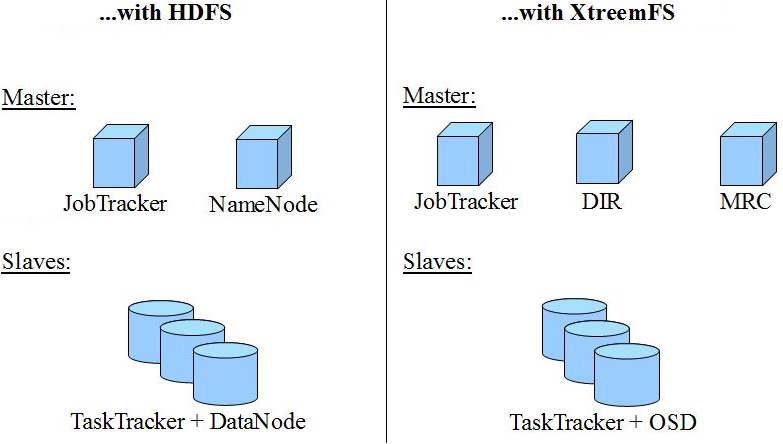
\includegraphics{images/cluster_setup.png}}
 % screenshot_status.png: 783x444 pixel, 72dpi, 28.82x29.88 cm, bb=0 0 783 444
 \caption{Hadoop cluster setup recommendation}
 \label{fig:cluster_setup}
\end{figure}

The three master services JobTracker, DIR and MRC are required in a Hadoop configuration. They can run alone or in arbitrary combinations on the same machine. Hadoop can be used with an arbitrary number of Slaves. It is recommended to run a TaskTracker together with an OSD on each Slave machine to improve performance, but it is not mandatory.

\section{Quick Start}
\label{sec:hadoop_quickstart}

This section will help you to set up a simple Hadoop configuration with all necessary services running on the same host.

\textbf{Required software:}
\begin{itemize}
\item XtreemFS servers (v 1.3.1) including XtreemFS.jar and Foundation.jar (\href{http://www.XtreemFS.org}{www.XtreemFS.org})
\item XtreemFSHadoopClient.jar (Download it from \href{http://code.google.com/p/xtreemfs/downloads/list}{www.XtreemFS.org} or build it by yourself by excecuting make hadoop-client)
\item Hadoop (v 1.0.1) (\href{http://hadoop.apache.org}{hadoop.apache.org})
\item JDK 1.6+ (\href{http://java.sun.com}{Oracle/SUN})
\end{itemize}

\textbf{Setup:}
\begin{enumerate}
 \item Install and start XtreemFS:\\
	Follow the instructions given by the quick start guide for XtreemFS, available at Sec.\ref{sec:quick_start}. Notice 	
	that the DIR is reachable at \textit{localhost:32638}, beause this information will be important later.

\item Download and extract Hadoop

\item Configure Hadoop to use XtreemFS instead of HDFS:
	\begin{enumerate}
	\item After downloading and extracting Hadoop you first have to add XtreemFS, the XtreemFSHadoopClient, ProtocolBuffer and the Foundation package to its 
	classpath. To do so edit the \textit{hadoop-env.sh} that can be found in the \textit{conf} directory of Hadoop and 
	add the paths to XtreemFS.jar, Foundation.jar, protobuf-java-2.3.0.jar and XtreemFSHadoopClient.jar separated by '\textit{:}' to the HADOOP\_CLASSPATH. 
	If you run a Linux-based OS these jar-libraries are located at '\textit{/usr/share/java/}'.
	For example
	\begin{verbatim}
	export HADOOP_CLASSPATH="/usr/share/java/Foundation.jar:
	/usr/share/java/XtreemFS.jar:/usr/share/XtreemFSHadoopClient.jar:
	/usr/share/java/protobuf-java-2.3.0.jar"
	\end{verbatim}
	should be sufficient on the most systems.
	\item Now you have to specify some properties at the \textit{core-site.xml} which also has to be in the \textit{conf} 
	directory of Hadoop. If this file does not exist you can safely create it.
	\begin{verbatim}
	<configuration>

		<property>
		  <name>fs.xtreemfs.impl</name>
		  <value>org.xtreemfs.common.clients.hadoop.XtreemFSFileSystem</value>
		  <description>The FileSystem for xtreemfs: uris.</description>
		</property>

		<property>
		  <name>fs.default.name</name>
		  <value>xtreemfs://localhost:32638</value>
		  <description>Address for the DIR.</description>
		</property>

		<property>
		  <name>xtreemfs.volumeName</name>
		  <value>volumeName</value>
		  <description>Name of the volume to use within XtreemFS.</description>
		</property>
		
		<property>
		  <name>io.file.buffer.size</name>
		  <value>131072</value>
		  <description>The size of buffer for use in sequence files 
		  in bytes.</description>
		</property>

	</configuration>
	\end{verbatim}
	\begin{enumerate}
	\item The first property is required to register the HadoopClient of XtreemFS at Hadoop. Now you are able to access 	
	XtreemFS by the Hadoop binary using the \textit{fs} argument. 
	\item The next property makes Hadoop use the DIR instead of a 
	NameNode, therefore address and port of the DIR has to be populated. In this case the DIR is located at 
	\textit{localhost:32638}. 
	\item The third property specifies the name of the volume to use within XtreemFS. Make sure, that the volume (here 
	named \textit{volumeName}) does exist. If the volume is not available Hadoop will not be able to use XtreemFS!
	\item The last property is tells Hadoop the size of buffers that will be used when reading/writing files.
	This size should be excatly the stripesize of your volume. Note that this value is measured in bytes while the
	stripe size of your volume usally is measured in kilo bytes. 
	\end{enumerate}
	Hint: If you want to provide userrights to your Hadoop installation according to the POSIX file-access-policy, you 
	have to set the following additional properties: 
	\begin{verbatim}
	<property>
	  <name>xtreemfs.client.userid</name>
	  <value>hadoopUserID</value>
	  <description>UserID to be used by Hadoop while accessing XtreemFS.</description>
	</property>

	<property>
	  <name>xtreemfs.client.groupid</name>
	  <value>hadoopGroupID</value>
	  <description>GroupID to be used by Hadoop while accessing XtreemFS.</description>
	</property>
	\end{verbatim}
	\end{enumerate}

\item To provide the minimum JobTracker configuration for Hadoop you have also to add the following property to the 
	\textit{conf/mapred-site.xml}:
	
	\begin{verbatim}
	<configuration>

	<property>
	  <name>mapred.job.tracker</name>
	  <value>localhost:9001</value>
	  <description>Listening address for the JobTracker.</description>
	</property>

	</configuration>
	\end{verbatim}
	Which specifies the address where the JobTracker will be running at.

\item Finally you are now able to start the JobTracker by running '\textit{bin/hadoop jobtracker}' from within the Hadoop root-directory and a TaskTracker by executing '\textit{bin/hadoop tasktracker}'.

\end{enumerate}
Congratulations! You successfully finished the quick start guide of the XtreemFS-Hadoop integration and are now able to use your Hadoop applications like as is well known or go on with the tutorials available on \href{http://hadoop.apache.org}{hadoop.apache.org}.

\chapter{Command Line Utilities}
\label{sec:cli_utils}

\begin{description}
 \item[lsfs.xtreemfs (formerly xtfs\_lsvol)] Lists the volumes on an MRC.
 \item[mkfs.xtreemfs (formerly xtfs\_mkvol)] Creates a new volume on an MRC.
 \item[mount.xtreemfs (formerly xtfs\_mount)] The XtreemFS client which mounts an XtreemFS volume locally on a machine.
 \item[rmfs.xtreemfs (formerly xtfs\_rmvol)] Deletes a volume.
 \item[umount.xtreemfs (formerly xtfs\_umount)] Un-mounts a mounted XtreemFS volume.
 \item[xstartserv] Tool for manually starting/stopping XtreemFS servers, e.g. for testing and development.
 \item[xtestenv] Tool for automatic set-up of a test environment and for executing the autotests.
 \item[xtfsutil] XtreemFS's swiss army knife.
 \item[xtfs\_cleanup] Deletes orphaned objects on an OSD, restores orphaned files and removes obsolete file versions.
 \item[xtfs\_chstatus] Changes the status of an service.
 \item[xtfs\_snap] Creates, lists and deletes snapshots.
 \item[xtfs\_mrcdbtool] Dumps and restores an XML representation of the MRC database.
 \item[xtfs\_remove\_osd] Relocates all files stored on an OSD in order to remove the OSD from the system.
 \item[xtfs\_scrub] Examines all files in a volume for wrong file sizes and checksums and corrects wrong file sizes in the MRC.
 \item[xtfs\_vivaldi] client service to calculate vivaldi coordinates.
\end{description}

\printindex

\end{document}
